% CVPR 2027 submission draft -- built on the official author kit (cvpr-org/author-kit, tag CVPR2027-v1).
\documentclass[10pt,twocolumn,letterpaper]{article}

%%%%%%%%% PAPER TYPE
\usepackage[review]{cvpr}      % REVIEW version (double-blind, line numbers)

%% Packages and macros shared by main.tex and supplement.tex.
%% Load before hyperref (cvpr.sty already loads amsmath, amssymb, booktabs, graphicx, xcolor, natbib, caption, subcaption).

\usepackage{cuted}      % two-column teaser (official kit tweak)
\usepackage{currfile}   % \currfilebase for figure labels (official kit tweak)
\usepackage{amsthm}
\usepackage{multirow}
\usepackage{tikz}
\usetikzlibrary{arrows.meta,positioning,fit,calc,backgrounds}

%% ---------------------------------------------------------------------------
%% Draft annotations. ALL of these must be gone (or switched off) before submission.
%%   \verify{...}   unverified fact / citation detail          (red)
%%   \pending{...}  number or sentence waiting for an experiment (red, bold)
%%   \tbd           empty table cell waiting for final numbers  (red dash)
%%   \TODO{...}     writing to-do                                (red, bold)
%%   \prelim{...}   preliminary (descriptive) number; rendered orange while \ifshowprelim is true
%% ---------------------------------------------------------------------------
\newif\ifshowprelim
\showprelimtrue   % set to \showprelimfalse to render preliminary numbers in black
\newcommand{\verify}[1]{{\color{red}[VERIFY: #1]}}
\newcommand{\pending}[1]{{\color{red}\textbf{[#1]}}}
\newcommand{\tbd}{{\color{red}--}}
\newcommand{\TODO}[1]{{\color{red}\textbf{[TODO: #1]}}}
\newcommand{\prelim}[1]{\ifshowprelim{\color{orange}#1}\else#1\fi}
%   \placeholder{title}{text}  framed box for an experiment that is still running (red frame)
\newcommand{\placeholder}[2]{\par\smallskip\noindent\fcolorbox{red}{red!3}{\parbox{\dimexpr\linewidth-2\fboxsep-2\fboxrule\relax}{\footnotesize\color{red!55!black}\textbf{[PLACEHOLDER: #1]} #2}}\par\smallskip}

%% ---------------------------------------------------------------------------
%% Envelope placement: THE single switch. \envelopemaintrue keeps Sec. 4.6 (and Prop. 2) in the main paper;
%% \envelopemainfalse moves them to Supp. D and leaves a one-sentence pointer, a limitation sentence and no
%% A-dual+env row in the main paper. Recompile both main.tex and supplement.tex after changing it.
%% ---------------------------------------------------------------------------
\newif\ifenvelopemain
\envelopemaintrue
\newcommand{\envref}{\ifenvelopemain\cref{sec:env}\else Supp.~D\fi}

%% ---------------------------------------------------------------------------
%% Method names (rename here only).
%% ---------------------------------------------------------------------------
\newcommand{\mDual}{\textsf{A-dual}\xspace}
\newcommand{\mDualBoth}{\textsf{A-dual-both}\xspace}
\newcommand{\mDualEnv}{\textsf{A-dual+env}\xspace}
\newcommand{\mDistSplit}{\textsf{A-dist-split}\xspace}
\newcommand{\mDistBoth}{\textsf{A-dist-both}\xspace}
\newcommand{\mLocal}{\textsf{A-local}\xspace}
\newcommand{\mLocalSplit}{\textsf{A-local-split}\xspace}
\newcommand{\mSplitCP}{\textsf{split-CP}\xspace}
\newcommand{\omnidc}{OMNI-DC\xspace}

%% ---------------------------------------------------------------------------
%% Notation.
%% ---------------------------------------------------------------------------
\newcommand{\yhat}{\hat{y}}
\newcommand{\ytil}{\tilde{y}}
\newcommand{\dtil}{\tilde{d}}
\newcommand{\cA}{\mathcal{A}}
\newcommand{\cP}{\mathcal{P}}
\newcommand{\cS}{\mathcal{S}}
\newcommand{\cQ}{\mathcal{Q}}
\newcommand{\cU}{\mathcal{U}}
\newcommand{\cE}{\mathcal{E}}
\newcommand{\cB}{\mathcal{B}}
\newcommand{\qhat}{\hat{q}}
\newcommand{\sg}{s_{\gamma}}
\newcommand{\Cov}{\mathrm{Cov}}
\newcommand{\E}{\mathbb{E}}
\renewcommand{\P}{\mathbb{P}}
\newcommand{\1}{\mathbf{1}}
\newcommand{\med}{\operatorname{med}}
\newcommand{\BetaBin}{\operatorname{BetaBin}}
\newcommand{\BetaD}{\operatorname{Beta}}

%% Theorem environments (numbered within the paper; the supplement restates them with the same numbers).
\theoremstyle{plain}
\newtheorem{theorem}{Theorem}
\newtheorem{proposition}{Proposition}
\newtheorem{lemma}{Lemma}
\theoremstyle{remark}
\newtheorem{remark}{Remark}

%% =====================================================================================
%% numbers.tex -- every experimental number used in the text, as a macro.
%%
%% Status tags in the comments:
%%   [theory]   follows from the method's definition (exact or Monte Carlo of a known law); final.
%%   [data]     dataset statistic; final unless the preprocessing changes.
%%   [prelim]   descriptive number from the exploratory runs (3 splits x 2 draws, gamma chosen after a
%%              first NYU/KITTI run). Rendered via \prelim{} (orange while drafting). MUST be replaced by
%%              the confirmatory replication (20 scene/visit splits, paired bootstrap, >= 10 probe draws,
%%              gamma frozen) before any superiority claim is printed.
%%   [pending]  not yet available; renders as a red placeholder via \pending{}.
%%
%% Source keys: "UPD" = docs/REPORT_UPDATE_2026-11-02.md, "REP" = docs/PROJECT_REPORT.md.
%% Model set caveat for every E17 [prelim] number on NYU/KITTI and ARKitScenes: the "six pairs" are
%% {NYU, KITTI} x {DA-V2, UniDepthV2, Depth Pro} (scripts/run_new.sh, E17_PAIRS default). This IS the paper's main
%% model set on NYU/KITTI; Metric3D v2 is supplement-only. Depth Pro is excluded on ARKitScenes only (not reproduced).
%% =====================================================================================

%% ---------- Motivation: scale error and structured-anchor failure (E11, E13) ----------
% REP 9.10 Finding 1 (E11, 5 seeds x 6 draws, six NYU/KITTI pairs incl. Depth Pro). [prelim]
\newcommand{\NumScaleVarLo}{\prelim{65}}
\newcommand{\NumScaleVarHi}{\prelim{79}}
% REP 9.16 (E13, 5 seeds x 3 draws): A-local coverage under clustered anchors, k = 20 and 200, range over pairs. [prelim]
\newcommand{\NumLocalClusterCovLo}{\prelim{0.26}}
\newcommand{\NumLocalClusterCovHi}{\prelim{0.47}}
% REP 9.16: A-local median relative width, clustered vs uniform anchors, k = 20. [prelim]
\newcommand{\NumLocalClusterWidthLo}{\prelim{0.020}}
\newcommand{\NumLocalClusterWidthHi}{\prelim{0.046}}
\newcommand{\NumLocalUnifWidthLo}{\prelim{0.15}}
\newcommand{\NumLocalUnifWidthHi}{\prelim{0.45}}
% REP 9.16: A-local coverage, near-only and scan-line (rows) layouts, range over pairs and k. [prelim]
\newcommand{\NumLocalNearCovLo}{\prelim{0.71}}
\newcommand{\NumLocalNearCovHi}{\prelim{0.79}}
\newcommand{\NumLocalRowsCovLo}{\prelim{0.87}}
\newcommand{\NumLocalRowsCovHi}{\prelim{0.89}}
% REP 7.4 (T8): A-local theoretical coverage with 20 uniform anchors (10 calibrate): 10/11. [theory]
\newcommand{\NumLocalTheoryTwenty}{0.909}
% REP 9.16 Finding 3: A-local, uniform anchors, k = 20: coverage next to an anchor (< 0.02 diag) vs beyond 0.2 diag. [prelim]
\newcommand{\NumLocalNearBinCovLo}{\prelim{0.93}}
\newcommand{\NumLocalNearBinCovHi}{\prelim{0.94}}
\newcommand{\NumLocalFarBinCovLo}{\prelim{0.61}}
\newcommand{\NumLocalFarBinCovHi}{\prelim{0.84}}

%% ---------- Dual-role calibration on NYU/KITTI (E17, UPD 9.22, job 46165) ----------
% UPD 9.22 Finding 2: A-dual median relative width vs A-dist-both, median over the six pairs, range over the
% 10 layout x k cells. [prelim]
\newcommand{\NumDualWidthGainLo}{\prelim{16}}
\newcommand{\NumDualWidthGainHi}{\prelim{69}}
% UPD 9.22: A-dual is >= 10 % narrower than A-dist-both on 6/6 pairs in every one of the 10 cells
% (the pre-registered method gate; coverage at its theoretical value). [prelim]
\newcommand{\NumDualGatePairs}{\prelim{6}}
\newcommand{\NumPairs}{6}
\newcommand{\NumCells}{10}
% UPD 9.22: A-dual image-averaged coverage, range over all cells (theory 19/21 = 0.905). [prelim]
\newcommand{\NumDualCovLo}{\prelim{0.902}}
\newcommand{\NumDualCovHi}{\prelim{0.907}}
% [theory] r/(n+1) with n = 20, alpha = 0.1: 19/21.
\newcommand{\NumDualCovTheory}{0.905}
% UPD 9.22: A-dual-both width vs A-dist-both (median over pairs, range over cells), gate cells passed,
% and interval score range over pairs (every pair, every cell). [prelim]
\newcommand{\NumDualBothWidthGainLo}{\prelim{2}}
\newcommand{\NumDualBothWidthGainHi}{\prelim{60}}
\newcommand{\NumDualBothCellsPass}{\prelim{8}}
\newcommand{\NumDualBothISGainLo}{\prelim{1}}
\newcommand{\NumDualBothISGainHi}{\prelim{48}}
% UPD 9.22: mean median relative widths over pairs and layouts, k = 50 / 200. [prelim]
\newcommand{\NumWDistSplitFifty}{\prelim{0.154}}
\newcommand{\NumWDistSplitTwoHundred}{\prelim{0.133}}
\newcommand{\NumWDualFifty}{\prelim{0.187}}
\newcommand{\NumWDualTwoHundred}{\prelim{0.161}}
\newcommand{\NumWDualBothFifty}{\prelim{0.225}}
\newcommand{\NumWDualBothTwoHundred}{\prelim{0.195}}
\newcommand{\NumWDistBothFifty}{\prelim{0.280}}
\newcommand{\NumWDistBothTwoHundred}{\prelim{0.281}}
% UPD 9.22: coverage A-dual-both / A-dist-both (means, k = 50). [prelim]
\newcommand{\NumCovDualBoth}{\prelim{0.959}}
\newcommand{\NumCovDistBoth}{\prelim{0.970}}
% UPD 9.22 Finding 5: coverage spread across distance bins holding >= 1 % of pixels, points, median over pairs,
% range over layout x k. [prelim]
\newcommand{\NumSpreadDualLo}{\prelim{3.9}}
\newcommand{\NumSpreadDualHi}{\prelim{12.3}}
\newcommand{\NumSpreadDualBothLo}{\prelim{1.3}}
\newcommand{\NumSpreadDualBothHi}{\prelim{2.2}}
% UPD 9.22 Finding 5: A-dual coverage, near layout k = 50, at 0.1-0.2 of the diagonal. [prelim]
\newcommand{\NumDualFarCov}{\prelim{0.81}}

%% ---------- Probe budget (T13 corollary) ----------
% [theory] Beta(r, n+1-r) large-population approximation of the exact beta-binomial law;
% p10 of single-draw per-image coverage, n = 10 / 20 / 40 (UPD 7.6; rechecked with scipy: 0.794/0.819/0.841).
\newcommand{\NumBetaPTenTen}{0.795}
\newcommand{\NumBetaPTenTwenty}{0.819}
\newcommand{\NumBetaPTenForty}{0.841}
% [theory] share of images below 0.85 when coverage is averaged over two independent probe draws (Monte Carlo).
\newcommand{\NumBetaShortTwoTen}{15.3}
\newcommand{\NumBetaShortTwoTwenty}{11.5}
\newcommand{\NumBetaShortTwoForty}{6.6}
% [theory] share below 0.85 for ONE probe draw (Beta CDF at 0.85): n = 10 / 20 / 40.
\newcommand{\NumBetaShortOneTen}{19.7}
\newcommand{\NumBetaShortOneTwenty}{17.6}
\newcommand{\NumBetaShortOneForty}{13.0}
% UPD 9.22 Finding 3: measured on NYU/KITTI (mean over pairs and layouts, k = 50) -- implementation check only. [prelim]
\newcommand{\NumMeasPTenTwenty}{\prelim{0.820}}
\newcommand{\NumMeasShortTwoTwenty}{\prelim{11.4}}

%% ---------- ARKitScenes (UPD 5, 9.23) ----------
% [data] depth-upsampling validation split after dropping one video without confidence maps.
\newcommand{\NumArkFrames}{5{,}594}
\newcommand{\NumArkVisits}{107}
\newcommand{\NumArkPixelsM}{23.8}
% [data] iPad vs Faro laser at drawn anchors: mean signed log error -0.0155 (iPad reads nearer).
\newcommand{\NumArkIpadOffset}{1.6}
% [data] share of pixels with ARKit confidence 2.
\newcommand{\NumArkConfTwo}{94.6}
% UPD 9.23 E0 (all frames). [prelim; final unless preprocessing changes]. Depth Pro aggregates deliberately omitted.
\newcommand{\NumArkUniAbsRel}{\prelim{0.120}}
\newcommand{\NumArkUniDeltaOne}{\prelim{0.882}}
\newcommand{\NumArkDavAbsRel}{\prelim{0.466}}
\newcommand{\NumArkDavDeltaOne}{\prelim{0.325}}
% UPD 9.22 Finding 3 (ARKitScenes, laser-valued probes, n = 20): short share (avg. of 2 draws) and p10.
% Recomputed 2 Nov WITHOUT Depth Pro: {DA-V2 indoor, UniDepthV2} x 5 layouts x k in {50, 200} (results/e17_p20_g05). [prelim]
\newcommand{\NumArkShortLo}{\prelim{10.5}}
\newcommand{\NumArkShortHi}{\prelim{12.1}}
\newcommand{\NumArkPTenLo}{\prelim{0.817}}
\newcommand{\NumArkPTenHi}{\prelim{0.821}}
% UPD 9.23 E16 (iPad-valued anchors, uniform, k = 200), UniDepthV2: within-image methods certify the sensor reading. [prelim]
\newcommand{\NumArkLocalIpadCovUni}{\prelim{0.854}}
\newcommand{\NumArkLscpIpadCovUni}{\prelim{0.548}}

%% ---------- E18: value-source factorial on ARKitScenes, frozen models, 20 seeds (running) ----------
% Uniform layout finished on the cluster, not yet pulled; cluster layout at 3/20 seeds.
% Truth coverage of A-dual, (structured-anchor source / probe source), uniform layout. [pending]
% NOTE: a 400-image smoke test gave ~0.52 truth coverage with iPad-valued probes -- do NOT print; wait for E18.
\newcommand{\NumEEighteenCovLL}{\pending{E18 cov.\ laser/laser}}
\newcommand{\NumEEighteenCovIL}{\pending{E18 cov.\ iPad/laser}}
\newcommand{\NumEEighteenCovLI}{\pending{E18 cov.\ laser/iPad}}
\newcommand{\NumEEighteenCovII}{\pending{E18 cov.\ iPad/iPad}}
% Sensor-error envelope (to run, CPU only). [pending]
\newcommand{\NumEnvTruthCov}{\pending{envelope truth cov.}}
\newcommand{\NumEnvISGain}{\pending{envelope IS gain vs \mDistBoth}}
\newcommand{\NumEnvAlphaS}{\pending{$\alpha_s$}}
\newcommand{\NumEnvAlphaE}{\pending{$\alpha_e$}}

%% ---------- E19: OMNI-DC centre on ARKitScenes (DONE, 3 seeds; exploratory) ----------
% results_omnidc/e19_summary_3seeds.csv: seeds 0-2 (visit splits), probe draw 0, k = 200 (180 structured + 20
% probes), alpha = 0.1, gamma = 0.5, UniDepthV2-L frozen; OMNI-DC v1.1 fed RGB + the 180 structured anchors.
% Table cells: \ENineteen{...} in the generated block below; derived text numbers: \NumOmni*, \NumCluster*, ...
\newcommand{\NumOmniSeeds}{3}
\newcommand{\NumOmniTestLo}{1{,}909}
\newcommand{\NumOmniTestHi}{1{,}945}
% Smoke test (8 images, NOT for the paper): AbsRel on unseen pixels ~0.6 % (180 uniform laser anchors),
% ~2.0 % (iPad anchors), ~4.3 % (clustered anchors). Full-set accuracy not yet computed. [pending]
\newcommand{\NumOmniAbsRelUniform}{\pending{OMNI-DC AbsRel, uniform}}
\newcommand{\NumOmniAbsRelCluster}{\pending{OMNI-DC AbsRel, cluster}}

%% ---------- Probe ablation n in {10, 40} (UPD 9.22 Finding 4) ----------
% A-dual median relative width, k = 50 / 200 (mean over pairs and layouts). [prelim]
\newcommand{\NumWDualTenFifty}{\prelim{0.202}}
\newcommand{\NumWDualTenTwoHundred}{\prelim{0.178}}
\newcommand{\NumWDualFortyFifty}{\prelim{0.199}}
\newcommand{\NumWDualFortyTwoHundred}{\prelim{0.154}}
% A-dual short share with 40 probes (two-draw mean), range over k. [prelim]
\newcommand{\NumShortFortyLo}{\prelim{6.5}}
\newcommand{\NumShortFortyHi}{\prelim{6.8}}

%% ---------- Table lookups (values in the generated block) ----------
\newcommand{\ESeventeen}[3]{\ifcsname e17/#1/#2/#3\endcsname\prelim{\csname e17/#1/#2/#3\endcsname}\else\pending{?}\fi}
\newcommand{\ENineteen}[6]{\ifcsname e19/#1/#2/#3/#4/#5/#6\endcsname\prelim{\csname e19/#1/#2/#3/#4/#5/#6\endcsname}\else\pending{?}\fi}

%% ---------- Confirmatory protocol (design, final) ----------
\newcommand{\NumReplSplits}{20}
\newcommand{\NumProbeDraws}{10}

%% >>> GENERATED by tools/gen_numbers.py -- do not edit by hand
%% E17 (Tab. 2): \ESeventeen{layout}{k}{col}; col in local, dual, short, dW, bW, bIS.
%% local/dual = image-averaged coverage of A-local (all k structured anchors) / A-dual; short = % images
%% with single-draw coverage < 0.85, A-dual (pending until frac_img_short exists); dW/bW = % change in
%% median rel. width of A-dual / A-dual-both vs A-dist-both; bIS = % change in rel. interval score
%% (primary if available), A-dual-both vs A-dist-both. Median over the six pairs; lo / hi = min / max.
\expandafter\def\csname e17/uniform/50/local\endcsname{0.922}
\expandafter\def\csname e17/uniform/50/locallo\endcsname{0.922}
\expandafter\def\csname e17/uniform/50/localhi\endcsname{0.924}
\expandafter\def\csname e17/uniform/50/dual\endcsname{0.905}
\expandafter\def\csname e17/uniform/50/duallo\endcsname{0.904}
\expandafter\def\csname e17/uniform/50/dualhi\endcsname{0.907}
\expandafter\def\csname e17/uniform/50/short\endcsname{\pending{confirmatory}}
\expandafter\def\csname e17/uniform/50/shortlo\endcsname{\pending{confirmatory}}
\expandafter\def\csname e17/uniform/50/shorthi\endcsname{\pending{confirmatory}}
\expandafter\def\csname e17/uniform/50/dW\endcsname{$-$48}
\expandafter\def\csname e17/uniform/50/dWlo\endcsname{$-$52}
\expandafter\def\csname e17/uniform/50/dWhi\endcsname{$-$45}
\expandafter\def\csname e17/uniform/50/bW\endcsname{$-$37}
\expandafter\def\csname e17/uniform/50/bWlo\endcsname{$-$42}
\expandafter\def\csname e17/uniform/50/bWhi\endcsname{$-$24}
\expandafter\def\csname e17/uniform/50/bIS\endcsname{$-$28}
\expandafter\def\csname e17/uniform/50/bISlo\endcsname{$-$30}
\expandafter\def\csname e17/uniform/50/bIShi\endcsname{$-$20}
\expandafter\def\csname e17/uniform/200/local\endcsname{0.901}
\expandafter\def\csname e17/uniform/200/locallo\endcsname{0.901}
\expandafter\def\csname e17/uniform/200/localhi\endcsname{0.902}
\expandafter\def\csname e17/uniform/200/dual\endcsname{0.906}
\expandafter\def\csname e17/uniform/200/duallo\endcsname{0.904}
\expandafter\def\csname e17/uniform/200/dualhi\endcsname{0.907}
\expandafter\def\csname e17/uniform/200/short\endcsname{\pending{confirmatory}}
\expandafter\def\csname e17/uniform/200/shortlo\endcsname{\pending{confirmatory}}
\expandafter\def\csname e17/uniform/200/shorthi\endcsname{\pending{confirmatory}}
\expandafter\def\csname e17/uniform/200/dW\endcsname{$-$69}
\expandafter\def\csname e17/uniform/200/dWlo\endcsname{$-$71}
\expandafter\def\csname e17/uniform/200/dWhi\endcsname{$-$61}
\expandafter\def\csname e17/uniform/200/bW\endcsname{$-$60}
\expandafter\def\csname e17/uniform/200/bWlo\endcsname{$-$67}
\expandafter\def\csname e17/uniform/200/bWhi\endcsname{$-$46}
\expandafter\def\csname e17/uniform/200/bIS\endcsname{$-$46}
\expandafter\def\csname e17/uniform/200/bISlo\endcsname{$-$48}
\expandafter\def\csname e17/uniform/200/bIShi\endcsname{$-$36}
\expandafter\def\csname e17/rows/50/local\endcsname{0.899}
\expandafter\def\csname e17/rows/50/locallo\endcsname{0.895}
\expandafter\def\csname e17/rows/50/localhi\endcsname{0.901}
\expandafter\def\csname e17/rows/50/dual\endcsname{0.905}
\expandafter\def\csname e17/rows/50/duallo\endcsname{0.903}
\expandafter\def\csname e17/rows/50/dualhi\endcsname{0.905}
\expandafter\def\csname e17/rows/50/short\endcsname{\pending{confirmatory}}
\expandafter\def\csname e17/rows/50/shortlo\endcsname{\pending{confirmatory}}
\expandafter\def\csname e17/rows/50/shorthi\endcsname{\pending{confirmatory}}
\expandafter\def\csname e17/rows/50/dW\endcsname{$-$41}
\expandafter\def\csname e17/rows/50/dWlo\endcsname{$-$45}
\expandafter\def\csname e17/rows/50/dWhi\endcsname{$-$38}
\expandafter\def\csname e17/rows/50/bW\endcsname{$-$30}
\expandafter\def\csname e17/rows/50/bWlo\endcsname{$-$34}
\expandafter\def\csname e17/rows/50/bWhi\endcsname{$-$20}
\expandafter\def\csname e17/rows/50/bIS\endcsname{$-$24}
\expandafter\def\csname e17/rows/50/bISlo\endcsname{$-$26}
\expandafter\def\csname e17/rows/50/bIShi\endcsname{$-$18}
\expandafter\def\csname e17/rows/200/local\endcsname{0.873}
\expandafter\def\csname e17/rows/200/locallo\endcsname{0.870}
\expandafter\def\csname e17/rows/200/localhi\endcsname{0.876}
\expandafter\def\csname e17/rows/200/dual\endcsname{0.904}
\expandafter\def\csname e17/rows/200/duallo\endcsname{0.902}
\expandafter\def\csname e17/rows/200/dualhi\endcsname{0.905}
\expandafter\def\csname e17/rows/200/short\endcsname{\pending{confirmatory}}
\expandafter\def\csname e17/rows/200/shortlo\endcsname{\pending{confirmatory}}
\expandafter\def\csname e17/rows/200/shorthi\endcsname{\pending{confirmatory}}
\expandafter\def\csname e17/rows/200/dW\endcsname{$-$53}
\expandafter\def\csname e17/rows/200/dWlo\endcsname{$-$58}
\expandafter\def\csname e17/rows/200/dWhi\endcsname{$-$48}
\expandafter\def\csname e17/rows/200/bW\endcsname{$-$44}
\expandafter\def\csname e17/rows/200/bWlo\endcsname{$-$47}
\expandafter\def\csname e17/rows/200/bWhi\endcsname{$-$32}
\expandafter\def\csname e17/rows/200/bIS\endcsname{$-$32}
\expandafter\def\csname e17/rows/200/bISlo\endcsname{$-$35}
\expandafter\def\csname e17/rows/200/bIShi\endcsname{$-$24}
\expandafter\def\csname e17/cluster/50/local\endcsname{0.342}
\expandafter\def\csname e17/cluster/50/locallo\endcsname{0.312}
\expandafter\def\csname e17/cluster/50/localhi\endcsname{0.412}
\expandafter\def\csname e17/cluster/50/dual\endcsname{0.906}
\expandafter\def\csname e17/cluster/50/duallo\endcsname{0.905}
\expandafter\def\csname e17/cluster/50/dualhi\endcsname{0.907}
\expandafter\def\csname e17/cluster/50/short\endcsname{\pending{confirmatory}}
\expandafter\def\csname e17/cluster/50/shortlo\endcsname{\pending{confirmatory}}
\expandafter\def\csname e17/cluster/50/shorthi\endcsname{\pending{confirmatory}}
\expandafter\def\csname e17/cluster/50/dW\endcsname{$-$16}
\expandafter\def\csname e17/cluster/50/dWlo\endcsname{$-$23}
\expandafter\def\csname e17/cluster/50/dWhi\endcsname{$-$10}
\expandafter\def\csname e17/cluster/50/bW\endcsname{$-$2}
\expandafter\def\csname e17/cluster/50/bWlo\endcsname{$-$4}
\expandafter\def\csname e17/cluster/50/bWhi\endcsname{0}
\expandafter\def\csname e17/cluster/50/bIS\endcsname{$-$1}
\expandafter\def\csname e17/cluster/50/bISlo\endcsname{$-$10}
\expandafter\def\csname e17/cluster/50/bIShi\endcsname{$-$1}
\expandafter\def\csname e17/cluster/200/local\endcsname{0.397}
\expandafter\def\csname e17/cluster/200/locallo\endcsname{0.366}
\expandafter\def\csname e17/cluster/200/localhi\endcsname{0.463}
\expandafter\def\csname e17/cluster/200/dual\endcsname{0.905}
\expandafter\def\csname e17/cluster/200/duallo\endcsname{0.903}
\expandafter\def\csname e17/cluster/200/dualhi\endcsname{0.905}
\expandafter\def\csname e17/cluster/200/short\endcsname{\pending{confirmatory}}
\expandafter\def\csname e17/cluster/200/shortlo\endcsname{\pending{confirmatory}}
\expandafter\def\csname e17/cluster/200/shorthi\endcsname{\pending{confirmatory}}
\expandafter\def\csname e17/cluster/200/dW\endcsname{$-$17}
\expandafter\def\csname e17/cluster/200/dWlo\endcsname{$-$24}
\expandafter\def\csname e17/cluster/200/dWhi\endcsname{$-$11}
\expandafter\def\csname e17/cluster/200/bW\endcsname{$-$3}
\expandafter\def\csname e17/cluster/200/bWlo\endcsname{$-$6}
\expandafter\def\csname e17/cluster/200/bWhi\endcsname{$-$0}
\expandafter\def\csname e17/cluster/200/bIS\endcsname{$-$4}
\expandafter\def\csname e17/cluster/200/bISlo\endcsname{$-$11}
\expandafter\def\csname e17/cluster/200/bIShi\endcsname{$-$1}
\expandafter\def\csname e17/edges/50/local\endcsname{0.960}
\expandafter\def\csname e17/edges/50/locallo\endcsname{0.939}
\expandafter\def\csname e17/edges/50/localhi\endcsname{0.967}
\expandafter\def\csname e17/edges/50/dual\endcsname{0.905}
\expandafter\def\csname e17/edges/50/duallo\endcsname{0.904}
\expandafter\def\csname e17/edges/50/dualhi\endcsname{0.906}
\expandafter\def\csname e17/edges/50/short\endcsname{\pending{confirmatory}}
\expandafter\def\csname e17/edges/50/shortlo\endcsname{\pending{confirmatory}}
\expandafter\def\csname e17/edges/50/shorthi\endcsname{\pending{confirmatory}}
\expandafter\def\csname e17/edges/50/dW\endcsname{$-$24}
\expandafter\def\csname e17/edges/50/dWlo\endcsname{$-$27}
\expandafter\def\csname e17/edges/50/dWhi\endcsname{$-$13}
\expandafter\def\csname e17/edges/50/bW\endcsname{$-$12}
\expandafter\def\csname e17/edges/50/bWlo\endcsname{$-$16}
\expandafter\def\csname e17/edges/50/bWhi\endcsname{$-$3}
\expandafter\def\csname e17/edges/50/bIS\endcsname{$-$15}
\expandafter\def\csname e17/edges/50/bISlo\endcsname{$-$16}
\expandafter\def\csname e17/edges/50/bIShi\endcsname{$-$6}
\expandafter\def\csname e17/edges/200/local\endcsname{0.948}
\expandafter\def\csname e17/edges/200/locallo\endcsname{0.922}
\expandafter\def\csname e17/edges/200/localhi\endcsname{0.960}
\expandafter\def\csname e17/edges/200/dual\endcsname{0.905}
\expandafter\def\csname e17/edges/200/duallo\endcsname{0.903}
\expandafter\def\csname e17/edges/200/dualhi\endcsname{0.905}
\expandafter\def\csname e17/edges/200/short\endcsname{\pending{confirmatory}}
\expandafter\def\csname e17/edges/200/shortlo\endcsname{\pending{confirmatory}}
\expandafter\def\csname e17/edges/200/shorthi\endcsname{\pending{confirmatory}}
\expandafter\def\csname e17/edges/200/dW\endcsname{$-$34}
\expandafter\def\csname e17/edges/200/dWlo\endcsname{$-$36}
\expandafter\def\csname e17/edges/200/dWhi\endcsname{$-$31}
\expandafter\def\csname e17/edges/200/bW\endcsname{$-$23}
\expandafter\def\csname e17/edges/200/bWlo\endcsname{$-$28}
\expandafter\def\csname e17/edges/200/bWhi\endcsname{$-$14}
\expandafter\def\csname e17/edges/200/bIS\endcsname{$-$18}
\expandafter\def\csname e17/edges/200/bISlo\endcsname{$-$25}
\expandafter\def\csname e17/edges/200/bIShi\endcsname{$-$17}
\expandafter\def\csname e17/near/50/local\endcsname{0.769}
\expandafter\def\csname e17/near/50/locallo\endcsname{0.754}
\expandafter\def\csname e17/near/50/localhi\endcsname{0.799}
\expandafter\def\csname e17/near/50/dual\endcsname{0.905}
\expandafter\def\csname e17/near/50/duallo\endcsname{0.904}
\expandafter\def\csname e17/near/50/dualhi\endcsname{0.906}
\expandafter\def\csname e17/near/50/short\endcsname{\pending{confirmatory}}
\expandafter\def\csname e17/near/50/shortlo\endcsname{\pending{confirmatory}}
\expandafter\def\csname e17/near/50/shorthi\endcsname{\pending{confirmatory}}
\expandafter\def\csname e17/near/50/dW\endcsname{$-$33}
\expandafter\def\csname e17/near/50/dWlo\endcsname{$-$46}
\expandafter\def\csname e17/near/50/dWhi\endcsname{$-$19}
\expandafter\def\csname e17/near/50/bW\endcsname{$-$18}
\expandafter\def\csname e17/near/50/bWlo\endcsname{$-$30}
\expandafter\def\csname e17/near/50/bWhi\endcsname{$-$11}
\expandafter\def\csname e17/near/50/bIS\endcsname{$-$18}
\expandafter\def\csname e17/near/50/bISlo\endcsname{$-$23}
\expandafter\def\csname e17/near/50/bIShi\endcsname{$-$14}
\expandafter\def\csname e17/near/200/local\endcsname{0.728}
\expandafter\def\csname e17/near/200/locallo\endcsname{0.712}
\expandafter\def\csname e17/near/200/localhi\endcsname{0.759}
\expandafter\def\csname e17/near/200/dual\endcsname{0.905}
\expandafter\def\csname e17/near/200/duallo\endcsname{0.903}
\expandafter\def\csname e17/near/200/dualhi\endcsname{0.906}
\expandafter\def\csname e17/near/200/short\endcsname{\pending{confirmatory}}
\expandafter\def\csname e17/near/200/shortlo\endcsname{\pending{confirmatory}}
\expandafter\def\csname e17/near/200/shorthi\endcsname{\pending{confirmatory}}
\expandafter\def\csname e17/near/200/dW\endcsname{$-$37}
\expandafter\def\csname e17/near/200/dWlo\endcsname{$-$52}
\expandafter\def\csname e17/near/200/dWhi\endcsname{$-$20}
\expandafter\def\csname e17/near/200/bW\endcsname{$-$22}
\expandafter\def\csname e17/near/200/bWlo\endcsname{$-$38}
\expandafter\def\csname e17/near/200/bWhi\endcsname{$-$12}
\expandafter\def\csname e17/near/200/bIS\endcsname{$-$20}
\expandafter\def\csname e17/near/200/bISlo\endcsname{$-$27}
\expandafter\def\csname e17/near/200/bIShi\endcsname{$-$13}
%% true while any E17 short cell is pending (Supp. ranges table then prints one marker, not [lo, hi])
\newif\ifESeventeenShortPending
\ESeventeenShortPendingtrue

%% E17 single-draw short share of A-dual (% images < 0.85, macro includes \%), range over pairs, layouts and k;
%% \pending{confirmatory} until the summaries carry frac_img_short (theory: 17.6 % at n = 20, 13.0 % at n = 40).
\newcommand{\NumESeventeenShort}{\pending{confirmatory}}
\newcommand{\NumESeventeenShortForty}{\pending{confirmatory}}
\newcommand{\NumArkShortOne}{\pending{confirmatory}}

%% E19 (Tab. 3, Supp.): \ENineteen{pattern}{centre}{anchor src}{probe src}{method}{col};
%% col in cov (truth coverage, image mean), ptten (p10 of per-image coverage, one draw), short (% images
%% < 0.85, one draw), wgt (median width / laser depth), is (rel. interval score: primary if the column
%% exists, else exploratory; then > 5.0 is a blow-up from a few pixels -> \pending),
%% uninf (% pixels with width > 10 y, only if frac_uninformative exists).
%% exploratory (seeds 0-2; not in the confirmatory E19c): cluster/omnidc/lidar/clean/A-dist-split, cluster/omnidc/lidar/clean/A-dual, cluster/omnidc/lidar/clean/A-dual-both, cluster/omnidc/lidar/clean/split-CP, cluster/omnidc/lidar/lidar/A-dist-split, cluster/omnidc/lidar/lidar/A-dual, cluster/omnidc/lidar/lidar/A-dual-both, cluster/omnidc/lidar/lidar/split-CP, uniform/omnidc/lidar/clean/A-dist-split, uniform/omnidc/lidar/clean/A-dual, uniform/omnidc/lidar/clean/A-dual-both, uniform/omnidc/lidar/clean/split-CP, uniform/omnidc/lidar/lidar/A-dist-split, uniform/omnidc/lidar/lidar/A-dual, uniform/omnidc/lidar/lidar/A-dual-both, uniform/omnidc/lidar/lidar/split-CP
\expandafter\def\csname e19/cluster/omnidc/clean/clean/A-dist-split/cov\endcsname{0.924}
\expandafter\def\csname e19/cluster/omnidc/clean/clean/A-dist-split/ptten\endcsname{0.757}
\expandafter\def\csname e19/cluster/omnidc/clean/clean/A-dist-split/short\endcsname{16.7}
\expandafter\def\csname e19/cluster/omnidc/clean/clean/A-dist-split/wgt\endcsname{0.391}
\expandafter\def\csname e19/cluster/omnidc/clean/clean/A-dist-split/is\endcsname{0.422}
\expandafter\def\csname e19/cluster/omnidc/clean/clean/A-dist-split/uninf\endcsname{0.2}
\expandafter\def\csname e19/cluster/omnidc/clean/clean/A-dual/cov\endcsname{0.905}
\expandafter\def\csname e19/cluster/omnidc/clean/clean/A-dual/ptten\endcsname{0.820}
\expandafter\def\csname e19/cluster/omnidc/clean/clean/A-dual/short\endcsname{17.4}
\expandafter\def\csname e19/cluster/omnidc/clean/clean/A-dual/wgt\endcsname{0.226}
\expandafter\def\csname e19/cluster/omnidc/clean/clean/A-dual/is\endcsname{0.311}
\expandafter\def\csname e19/cluster/omnidc/clean/clean/A-dual/uninf\endcsname{0.0}
\expandafter\def\csname e19/cluster/omnidc/clean/clean/A-dual-both/cov\endcsname{0.971}
\expandafter\def\csname e19/cluster/omnidc/clean/clean/A-dual-both/ptten\endcsname{0.917}
\expandafter\def\csname e19/cluster/omnidc/clean/clean/A-dual-both/short\endcsname{2.2}
\expandafter\def\csname e19/cluster/omnidc/clean/clean/A-dual-both/wgt\endcsname{0.403}
\expandafter\def\csname e19/cluster/omnidc/clean/clean/A-dual-both/is\endcsname{0.421}
\expandafter\def\csname e19/cluster/omnidc/clean/clean/A-dual-both/uninf\endcsname{0.2}
\expandafter\def\csname e19/cluster/omnidc/clean/clean/split-CP/cov\endcsname{0.895}
\expandafter\def\csname e19/cluster/omnidc/clean/clean/split-CP/ptten\endcsname{0.676}
\expandafter\def\csname e19/cluster/omnidc/clean/clean/split-CP/short\endcsname{23.7}
\expandafter\def\csname e19/cluster/omnidc/clean/clean/split-CP/wgt\endcsname{0.336}
\expandafter\def\csname e19/cluster/omnidc/clean/clean/split-CP/is\endcsname{0.374}
\expandafter\def\csname e19/cluster/omnidc/clean/clean/split-CP/uninf\endcsname{0.0}
\expandafter\def\csname e19/cluster/omnidc/clean/lidar/A-dist-split/cov\endcsname{0.924}
\expandafter\def\csname e19/cluster/omnidc/clean/lidar/A-dist-split/ptten\endcsname{0.757}
\expandafter\def\csname e19/cluster/omnidc/clean/lidar/A-dist-split/short\endcsname{16.7}
\expandafter\def\csname e19/cluster/omnidc/clean/lidar/A-dist-split/wgt\endcsname{0.391}
\expandafter\def\csname e19/cluster/omnidc/clean/lidar/A-dist-split/is\endcsname{0.422}
\expandafter\def\csname e19/cluster/omnidc/clean/lidar/A-dist-split/uninf\endcsname{0.2}
\expandafter\def\csname e19/cluster/omnidc/clean/lidar/A-dual/cov\endcsname{0.915}
\expandafter\def\csname e19/cluster/omnidc/clean/lidar/A-dual/ptten\endcsname{0.807}
\expandafter\def\csname e19/cluster/omnidc/clean/lidar/A-dual/short\endcsname{17.4}
\expandafter\def\csname e19/cluster/omnidc/clean/lidar/A-dual/wgt\endcsname{0.241}
\expandafter\def\csname e19/cluster/omnidc/clean/lidar/A-dual/is\endcsname{0.322}
\expandafter\def\csname e19/cluster/omnidc/clean/lidar/A-dual/uninf\endcsname{0.0}
\expandafter\def\csname e19/cluster/omnidc/clean/lidar/A-dual-both/cov\endcsname{0.971}
\expandafter\def\csname e19/cluster/omnidc/clean/lidar/A-dual-both/ptten\endcsname{0.912}
\expandafter\def\csname e19/cluster/omnidc/clean/lidar/A-dual-both/short\endcsname{3.1}
\expandafter\def\csname e19/cluster/omnidc/clean/lidar/A-dual-both/wgt\endcsname{0.403}
\expandafter\def\csname e19/cluster/omnidc/clean/lidar/A-dual-both/is\endcsname{0.423}
\expandafter\def\csname e19/cluster/omnidc/clean/lidar/A-dual-both/uninf\endcsname{0.2}
\expandafter\def\csname e19/cluster/omnidc/clean/lidar/split-CP/cov\endcsname{0.895}
\expandafter\def\csname e19/cluster/omnidc/clean/lidar/split-CP/ptten\endcsname{0.676}
\expandafter\def\csname e19/cluster/omnidc/clean/lidar/split-CP/short\endcsname{23.7}
\expandafter\def\csname e19/cluster/omnidc/clean/lidar/split-CP/wgt\endcsname{0.336}
\expandafter\def\csname e19/cluster/omnidc/clean/lidar/split-CP/is\endcsname{0.374}
\expandafter\def\csname e19/cluster/omnidc/clean/lidar/split-CP/uninf\endcsname{0.0}
\expandafter\def\csname e19/cluster/omnidc/lidar/clean/A-dist-split/cov\endcsname{0.922}
\expandafter\def\csname e19/cluster/omnidc/lidar/clean/A-dist-split/ptten\endcsname{0.747}
\expandafter\def\csname e19/cluster/omnidc/lidar/clean/A-dist-split/short\endcsname{17.2}
\expandafter\def\csname e19/cluster/omnidc/lidar/clean/A-dist-split/wgt\endcsname{0.391}
\expandafter\def\csname e19/cluster/omnidc/lidar/clean/A-dist-split/is\endcsname{0.589}
\expandafter\def\csname e19/cluster/omnidc/lidar/clean/A-dist-split/uninf\endcsname{--}
\expandafter\def\csname e19/cluster/omnidc/lidar/clean/A-dual/cov\endcsname{0.905}
\expandafter\def\csname e19/cluster/omnidc/lidar/clean/A-dual/ptten\endcsname{0.820}
\expandafter\def\csname e19/cluster/omnidc/lidar/clean/A-dual/short\endcsname{17.2}
\expandafter\def\csname e19/cluster/omnidc/lidar/clean/A-dual/wgt\endcsname{0.233}
\expandafter\def\csname e19/cluster/omnidc/lidar/clean/A-dual/is\endcsname{\pending{primary IS}} % mean 8.75e+03: blow-up
\expandafter\def\csname e19/cluster/omnidc/lidar/clean/A-dual/uninf\endcsname{--}
\expandafter\def\csname e19/cluster/omnidc/lidar/clean/A-dual-both/cov\endcsname{0.971}
\expandafter\def\csname e19/cluster/omnidc/lidar/clean/A-dual-both/ptten\endcsname{0.918}
\expandafter\def\csname e19/cluster/omnidc/lidar/clean/A-dual-both/short\endcsname{2.2}
\expandafter\def\csname e19/cluster/omnidc/lidar/clean/A-dual-both/wgt\endcsname{0.404}
\expandafter\def\csname e19/cluster/omnidc/lidar/clean/A-dual-both/is\endcsname{\pending{primary IS}} % mean 8.75e+03: blow-up
\expandafter\def\csname e19/cluster/omnidc/lidar/clean/A-dual-both/uninf\endcsname{--}
\expandafter\def\csname e19/cluster/omnidc/lidar/clean/split-CP/cov\endcsname{0.894}
\expandafter\def\csname e19/cluster/omnidc/lidar/clean/split-CP/ptten\endcsname{0.665}
\expandafter\def\csname e19/cluster/omnidc/lidar/clean/split-CP/short\endcsname{24.3}
\expandafter\def\csname e19/cluster/omnidc/lidar/clean/split-CP/wgt\endcsname{0.336}
\expandafter\def\csname e19/cluster/omnidc/lidar/clean/split-CP/is\endcsname{0.581}
\expandafter\def\csname e19/cluster/omnidc/lidar/clean/split-CP/uninf\endcsname{--}
\expandafter\def\csname e19/cluster/omnidc/lidar/lidar/A-dist-split/cov\endcsname{0.922}
\expandafter\def\csname e19/cluster/omnidc/lidar/lidar/A-dist-split/ptten\endcsname{0.747}
\expandafter\def\csname e19/cluster/omnidc/lidar/lidar/A-dist-split/short\endcsname{17.2}
\expandafter\def\csname e19/cluster/omnidc/lidar/lidar/A-dist-split/wgt\endcsname{0.391}
\expandafter\def\csname e19/cluster/omnidc/lidar/lidar/A-dist-split/is\endcsname{0.589}
\expandafter\def\csname e19/cluster/omnidc/lidar/lidar/A-dist-split/uninf\endcsname{--}
\expandafter\def\csname e19/cluster/omnidc/lidar/lidar/A-dual/cov\endcsname{0.881}
\expandafter\def\csname e19/cluster/omnidc/lidar/lidar/A-dual/ptten\endcsname{0.737}
\expandafter\def\csname e19/cluster/omnidc/lidar/lidar/A-dual/short\endcsname{29.7}
\expandafter\def\csname e19/cluster/omnidc/lidar/lidar/A-dual/wgt\endcsname{0.227}
\expandafter\def\csname e19/cluster/omnidc/lidar/lidar/A-dual/is\endcsname{\pending{primary IS}} % mean 1e+04: blow-up
\expandafter\def\csname e19/cluster/omnidc/lidar/lidar/A-dual/uninf\endcsname{--}
\expandafter\def\csname e19/cluster/omnidc/lidar/lidar/A-dual-both/cov\endcsname{0.968}
\expandafter\def\csname e19/cluster/omnidc/lidar/lidar/A-dual-both/ptten\endcsname{0.904}
\expandafter\def\csname e19/cluster/omnidc/lidar/lidar/A-dual-both/short\endcsname{3.9}
\expandafter\def\csname e19/cluster/omnidc/lidar/lidar/A-dual-both/wgt\endcsname{0.403}
\expandafter\def\csname e19/cluster/omnidc/lidar/lidar/A-dual-both/is\endcsname{\pending{primary IS}} % mean 1e+04: blow-up
\expandafter\def\csname e19/cluster/omnidc/lidar/lidar/A-dual-both/uninf\endcsname{--}
\expandafter\def\csname e19/cluster/omnidc/lidar/lidar/split-CP/cov\endcsname{0.894}
\expandafter\def\csname e19/cluster/omnidc/lidar/lidar/split-CP/ptten\endcsname{0.665}
\expandafter\def\csname e19/cluster/omnidc/lidar/lidar/split-CP/short\endcsname{24.3}
\expandafter\def\csname e19/cluster/omnidc/lidar/lidar/split-CP/wgt\endcsname{0.336}
\expandafter\def\csname e19/cluster/omnidc/lidar/lidar/split-CP/is\endcsname{0.581}
\expandafter\def\csname e19/cluster/omnidc/lidar/lidar/split-CP/uninf\endcsname{--}
\expandafter\def\csname e19/cluster/unidepth/clean/clean/A-dist-split/cov\endcsname{0.924}
\expandafter\def\csname e19/cluster/unidepth/clean/clean/A-dist-split/ptten\endcsname{0.837}
\expandafter\def\csname e19/cluster/unidepth/clean/clean/A-dist-split/short\endcsname{12.5}
\expandafter\def\csname e19/cluster/unidepth/clean/clean/A-dist-split/wgt\endcsname{0.071}
\expandafter\def\csname e19/cluster/unidepth/clean/clean/A-dist-split/is\endcsname{0.135}
\expandafter\def\csname e19/cluster/unidepth/clean/clean/A-dist-split/uninf\endcsname{0.0}
\expandafter\def\csname e19/cluster/unidepth/clean/clean/A-dual/cov\endcsname{0.905}
\expandafter\def\csname e19/cluster/unidepth/clean/clean/A-dual/ptten\endcsname{0.819}
\expandafter\def\csname e19/cluster/unidepth/clean/clean/A-dual/short\endcsname{17.6}
\expandafter\def\csname e19/cluster/unidepth/clean/clean/A-dual/wgt\endcsname{0.109}
\expandafter\def\csname e19/cluster/unidepth/clean/clean/A-dual/is\endcsname{0.182}
\expandafter\def\csname e19/cluster/unidepth/clean/clean/A-dual/uninf\endcsname{0.0}
\expandafter\def\csname e19/cluster/unidepth/clean/clean/A-dual-both/cov\endcsname{0.967}
\expandafter\def\csname e19/cluster/unidepth/clean/clean/A-dual-both/ptten\endcsname{0.930}
\expandafter\def\csname e19/cluster/unidepth/clean/clean/A-dual-both/short\endcsname{0.5}
\expandafter\def\csname e19/cluster/unidepth/clean/clean/A-dual-both/wgt\endcsname{0.126}
\expandafter\def\csname e19/cluster/unidepth/clean/clean/A-dual-both/is\endcsname{0.174}
\expandafter\def\csname e19/cluster/unidepth/clean/clean/A-dual-both/uninf\endcsname{0.0}
\expandafter\def\csname e19/cluster/unidepth/clean/clean/split-CP/cov\endcsname{0.897}
\expandafter\def\csname e19/cluster/unidepth/clean/clean/split-CP/ptten\endcsname{0.595}
\expandafter\def\csname e19/cluster/unidepth/clean/clean/split-CP/short\endcsname{14.6}
\expandafter\def\csname e19/cluster/unidepth/clean/clean/split-CP/wgt\endcsname{0.513}
\expandafter\def\csname e19/cluster/unidepth/clean/clean/split-CP/is\endcsname{0.529}
\expandafter\def\csname e19/cluster/unidepth/clean/clean/split-CP/uninf\endcsname{0.0}
\expandafter\def\csname e19/cluster/unidepth/clean/lidar/A-dist-split/cov\endcsname{0.925}
\expandafter\def\csname e19/cluster/unidepth/clean/lidar/A-dist-split/ptten\endcsname{0.840}
\expandafter\def\csname e19/cluster/unidepth/clean/lidar/A-dist-split/short\endcsname{12.0}
\expandafter\def\csname e19/cluster/unidepth/clean/lidar/A-dist-split/wgt\endcsname{0.090}
\expandafter\def\csname e19/cluster/unidepth/clean/lidar/A-dist-split/is\endcsname{0.152}
\expandafter\def\csname e19/cluster/unidepth/clean/lidar/A-dist-split/uninf\endcsname{0.0}
\expandafter\def\csname e19/cluster/unidepth/clean/lidar/A-dual/cov\endcsname{0.927}
\expandafter\def\csname e19/cluster/unidepth/clean/lidar/A-dual/ptten\endcsname{0.823}
\expandafter\def\csname e19/cluster/unidepth/clean/lidar/A-dual/short\endcsname{13.3}
\expandafter\def\csname e19/cluster/unidepth/clean/lidar/A-dual/wgt\endcsname{0.131}
\expandafter\def\csname e19/cluster/unidepth/clean/lidar/A-dual/is\endcsname{0.197}
\expandafter\def\csname e19/cluster/unidepth/clean/lidar/A-dual/uninf\endcsname{0.0}
\expandafter\def\csname e19/cluster/unidepth/clean/lidar/A-dual-both/cov\endcsname{0.971}
\expandafter\def\csname e19/cluster/unidepth/clean/lidar/A-dual-both/ptten\endcsname{0.932}
\expandafter\def\csname e19/cluster/unidepth/clean/lidar/A-dual-both/short\endcsname{0.9}
\expandafter\def\csname e19/cluster/unidepth/clean/lidar/A-dual-both/wgt\endcsname{0.148}
\expandafter\def\csname e19/cluster/unidepth/clean/lidar/A-dual-both/is\endcsname{0.193}
\expandafter\def\csname e19/cluster/unidepth/clean/lidar/A-dual-both/uninf\endcsname{0.0}
\expandafter\def\csname e19/cluster/unidepth/clean/lidar/split-CP/cov\endcsname{0.897}
\expandafter\def\csname e19/cluster/unidepth/clean/lidar/split-CP/ptten\endcsname{0.595}
\expandafter\def\csname e19/cluster/unidepth/clean/lidar/split-CP/short\endcsname{14.6}
\expandafter\def\csname e19/cluster/unidepth/clean/lidar/split-CP/wgt\endcsname{0.513}
\expandafter\def\csname e19/cluster/unidepth/clean/lidar/split-CP/is\endcsname{0.529}
\expandafter\def\csname e19/cluster/unidepth/clean/lidar/split-CP/uninf\endcsname{0.0}
\expandafter\def\csname e19/cluster/unidepth/lidar/clean/A-dist-split/cov\endcsname{0.942}
\expandafter\def\csname e19/cluster/unidepth/lidar/clean/A-dist-split/ptten\endcsname{0.868}
\expandafter\def\csname e19/cluster/unidepth/lidar/clean/A-dist-split/short\endcsname{7.0}
\expandafter\def\csname e19/cluster/unidepth/lidar/clean/A-dist-split/wgt\endcsname{0.098}
\expandafter\def\csname e19/cluster/unidepth/lidar/clean/A-dist-split/is\endcsname{0.152}
\expandafter\def\csname e19/cluster/unidepth/lidar/clean/A-dist-split/uninf\endcsname{0.0}
\expandafter\def\csname e19/cluster/unidepth/lidar/clean/A-dual/cov\endcsname{0.906}
\expandafter\def\csname e19/cluster/unidepth/lidar/clean/A-dual/ptten\endcsname{0.820}
\expandafter\def\csname e19/cluster/unidepth/lidar/clean/A-dual/short\endcsname{17.5}
\expandafter\def\csname e19/cluster/unidepth/lidar/clean/A-dual/wgt\endcsname{0.123}
\expandafter\def\csname e19/cluster/unidepth/lidar/clean/A-dual/is\endcsname{0.191}
\expandafter\def\csname e19/cluster/unidepth/lidar/clean/A-dual/uninf\endcsname{0.0}
\expandafter\def\csname e19/cluster/unidepth/lidar/clean/A-dual-both/cov\endcsname{0.972}
\expandafter\def\csname e19/cluster/unidepth/lidar/clean/A-dual-both/ptten\endcsname{0.938}
\expandafter\def\csname e19/cluster/unidepth/lidar/clean/A-dual-both/short\endcsname{0.3}
\expandafter\def\csname e19/cluster/unidepth/lidar/clean/A-dual-both/wgt\endcsname{0.146}
\expandafter\def\csname e19/cluster/unidepth/lidar/clean/A-dual-both/is\endcsname{0.188}
\expandafter\def\csname e19/cluster/unidepth/lidar/clean/A-dual-both/uninf\endcsname{0.0}
\expandafter\def\csname e19/cluster/unidepth/lidar/clean/split-CP/cov\endcsname{0.897}
\expandafter\def\csname e19/cluster/unidepth/lidar/clean/split-CP/ptten\endcsname{0.595}
\expandafter\def\csname e19/cluster/unidepth/lidar/clean/split-CP/short\endcsname{14.6}
\expandafter\def\csname e19/cluster/unidepth/lidar/clean/split-CP/wgt\endcsname{0.513}
\expandafter\def\csname e19/cluster/unidepth/lidar/clean/split-CP/is\endcsname{0.529}
\expandafter\def\csname e19/cluster/unidepth/lidar/clean/split-CP/uninf\endcsname{0.0}
\expandafter\def\csname e19/cluster/unidepth/lidar/lidar/A-dist-split/cov\endcsname{0.866}
\expandafter\def\csname e19/cluster/unidepth/lidar/lidar/A-dist-split/ptten\endcsname{0.746}
\expandafter\def\csname e19/cluster/unidepth/lidar/lidar/A-dist-split/short\endcsname{33.0}
\expandafter\def\csname e19/cluster/unidepth/lidar/lidar/A-dist-split/wgt\endcsname{0.081}
\expandafter\def\csname e19/cluster/unidepth/lidar/lidar/A-dist-split/is\endcsname{0.157}
\expandafter\def\csname e19/cluster/unidepth/lidar/lidar/A-dist-split/uninf\endcsname{0.0}
\expandafter\def\csname e19/cluster/unidepth/lidar/lidar/A-dual/cov\endcsname{0.848}
\expandafter\def\csname e19/cluster/unidepth/lidar/lidar/A-dual/ptten\endcsname{0.623}
\expandafter\def\csname e19/cluster/unidepth/lidar/lidar/A-dual/short\endcsname{33.6}
\expandafter\def\csname e19/cluster/unidepth/lidar/lidar/A-dual/wgt\endcsname{0.119}
\expandafter\def\csname e19/cluster/unidepth/lidar/lidar/A-dual/is\endcsname{0.209}
\expandafter\def\csname e19/cluster/unidepth/lidar/lidar/A-dual/uninf\endcsname{0.0}
\expandafter\def\csname e19/cluster/unidepth/lidar/lidar/A-dual-both/cov\endcsname{0.946}
\expandafter\def\csname e19/cluster/unidepth/lidar/lidar/A-dual-both/ptten\endcsname{0.882}
\expandafter\def\csname e19/cluster/unidepth/lidar/lidar/A-dual-both/short\endcsname{6.0}
\expandafter\def\csname e19/cluster/unidepth/lidar/lidar/A-dual-both/wgt\endcsname{0.137}
\expandafter\def\csname e19/cluster/unidepth/lidar/lidar/A-dual-both/is\endcsname{0.189}
\expandafter\def\csname e19/cluster/unidepth/lidar/lidar/A-dual-both/uninf\endcsname{0.0}
\expandafter\def\csname e19/cluster/unidepth/lidar/lidar/split-CP/cov\endcsname{0.897}
\expandafter\def\csname e19/cluster/unidepth/lidar/lidar/split-CP/ptten\endcsname{0.595}
\expandafter\def\csname e19/cluster/unidepth/lidar/lidar/split-CP/short\endcsname{14.6}
\expandafter\def\csname e19/cluster/unidepth/lidar/lidar/split-CP/wgt\endcsname{0.513}
\expandafter\def\csname e19/cluster/unidepth/lidar/lidar/split-CP/is\endcsname{0.529}
\expandafter\def\csname e19/cluster/unidepth/lidar/lidar/split-CP/uninf\endcsname{0.0}
\expandafter\def\csname e19/uniform/omnidc/clean/clean/A-dist-split/cov\endcsname{0.923}
\expandafter\def\csname e19/uniform/omnidc/clean/clean/A-dist-split/ptten\endcsname{0.850}
\expandafter\def\csname e19/uniform/omnidc/clean/clean/A-dist-split/short\endcsname{9.9}
\expandafter\def\csname e19/uniform/omnidc/clean/clean/A-dist-split/wgt\endcsname{0.026}
\expandafter\def\csname e19/uniform/omnidc/clean/clean/A-dist-split/is\endcsname{0.071}
\expandafter\def\csname e19/uniform/omnidc/clean/clean/A-dist-split/uninf\endcsname{0.0}
\expandafter\def\csname e19/uniform/omnidc/clean/clean/A-dual/cov\endcsname{0.904}
\expandafter\def\csname e19/uniform/omnidc/clean/clean/A-dual/ptten\endcsname{0.819}
\expandafter\def\csname e19/uniform/omnidc/clean/clean/A-dual/short\endcsname{17.8}
\expandafter\def\csname e19/uniform/omnidc/clean/clean/A-dual/wgt\endcsname{0.023}
\expandafter\def\csname e19/uniform/omnidc/clean/clean/A-dual/is\endcsname{0.074}
\expandafter\def\csname e19/uniform/omnidc/clean/clean/A-dual/uninf\endcsname{0.0}
\expandafter\def\csname e19/uniform/omnidc/clean/clean/A-dual-both/cov\endcsname{0.948}
\expandafter\def\csname e19/uniform/omnidc/clean/clean/A-dual-both/ptten\endcsname{0.902}
\expandafter\def\csname e19/uniform/omnidc/clean/clean/A-dual-both/short\endcsname{1.3}
\expandafter\def\csname e19/uniform/omnidc/clean/clean/A-dual-both/wgt\endcsname{0.032}
\expandafter\def\csname e19/uniform/omnidc/clean/clean/A-dual-both/is\endcsname{0.074}
\expandafter\def\csname e19/uniform/omnidc/clean/clean/A-dual-both/uninf\endcsname{0.0}
\expandafter\def\csname e19/uniform/omnidc/clean/clean/split-CP/cov\endcsname{0.897}
\expandafter\def\csname e19/uniform/omnidc/clean/clean/split-CP/ptten\endcsname{0.813}
\expandafter\def\csname e19/uniform/omnidc/clean/clean/split-CP/short\endcsname{20.7}
\expandafter\def\csname e19/uniform/omnidc/clean/clean/split-CP/wgt\endcsname{0.024}
\expandafter\def\csname e19/uniform/omnidc/clean/clean/split-CP/is\endcsname{0.073}
\expandafter\def\csname e19/uniform/omnidc/clean/clean/split-CP/uninf\endcsname{0.0}
\expandafter\def\csname e19/uniform/omnidc/clean/lidar/A-dist-split/cov\endcsname{0.923}
\expandafter\def\csname e19/uniform/omnidc/clean/lidar/A-dist-split/ptten\endcsname{0.851}
\expandafter\def\csname e19/uniform/omnidc/clean/lidar/A-dist-split/short\endcsname{9.9}
\expandafter\def\csname e19/uniform/omnidc/clean/lidar/A-dist-split/wgt\endcsname{0.026}
\expandafter\def\csname e19/uniform/omnidc/clean/lidar/A-dist-split/is\endcsname{0.071}
\expandafter\def\csname e19/uniform/omnidc/clean/lidar/A-dist-split/uninf\endcsname{0.0}
\expandafter\def\csname e19/uniform/omnidc/clean/lidar/A-dual/cov\endcsname{0.980}
\expandafter\def\csname e19/uniform/omnidc/clean/lidar/A-dual/ptten\endcsname{0.956}
\expandafter\def\csname e19/uniform/omnidc/clean/lidar/A-dual/short\endcsname{0.0}
\expandafter\def\csname e19/uniform/omnidc/clean/lidar/A-dual/wgt\endcsname{0.075}
\expandafter\def\csname e19/uniform/omnidc/clean/lidar/A-dual/is\endcsname{0.108}
\expandafter\def\csname e19/uniform/omnidc/clean/lidar/A-dual/uninf\endcsname{0.0}
\expandafter\def\csname e19/uniform/omnidc/clean/lidar/A-dual-both/cov\endcsname{0.980}
\expandafter\def\csname e19/uniform/omnidc/clean/lidar/A-dual-both/ptten\endcsname{0.957}
\expandafter\def\csname e19/uniform/omnidc/clean/lidar/A-dual-both/short\endcsname{0.0}
\expandafter\def\csname e19/uniform/omnidc/clean/lidar/A-dual-both/wgt\endcsname{0.075}
\expandafter\def\csname e19/uniform/omnidc/clean/lidar/A-dual-both/is\endcsname{0.108}
\expandafter\def\csname e19/uniform/omnidc/clean/lidar/A-dual-both/uninf\endcsname{0.0}
\expandafter\def\csname e19/uniform/omnidc/clean/lidar/split-CP/cov\endcsname{0.897}
\expandafter\def\csname e19/uniform/omnidc/clean/lidar/split-CP/ptten\endcsname{0.813}
\expandafter\def\csname e19/uniform/omnidc/clean/lidar/split-CP/short\endcsname{20.7}
\expandafter\def\csname e19/uniform/omnidc/clean/lidar/split-CP/wgt\endcsname{0.024}
\expandafter\def\csname e19/uniform/omnidc/clean/lidar/split-CP/is\endcsname{0.073}
\expandafter\def\csname e19/uniform/omnidc/clean/lidar/split-CP/uninf\endcsname{0.0}
\expandafter\def\csname e19/uniform/omnidc/lidar/clean/A-dist-split/cov\endcsname{0.545}
\expandafter\def\csname e19/uniform/omnidc/lidar/clean/A-dist-split/ptten\endcsname{0.330}
\expandafter\def\csname e19/uniform/omnidc/lidar/clean/A-dist-split/short\endcsname{97.9}
\expandafter\def\csname e19/uniform/omnidc/lidar/clean/A-dist-split/wgt\endcsname{0.036}
\expandafter\def\csname e19/uniform/omnidc/lidar/clean/A-dist-split/is\endcsname{0.199}
\expandafter\def\csname e19/uniform/omnidc/lidar/clean/A-dist-split/uninf\endcsname{--}
\expandafter\def\csname e19/uniform/omnidc/lidar/clean/A-dual/cov\endcsname{0.905}
\expandafter\def\csname e19/uniform/omnidc/lidar/clean/A-dual/ptten\endcsname{0.817}
\expandafter\def\csname e19/uniform/omnidc/lidar/clean/A-dual/short\endcsname{18.4}
\expandafter\def\csname e19/uniform/omnidc/lidar/clean/A-dual/wgt\endcsname{0.071}
\expandafter\def\csname e19/uniform/omnidc/lidar/clean/A-dual/is\endcsname{0.150}
\expandafter\def\csname e19/uniform/omnidc/lidar/clean/A-dual/uninf\endcsname{--}
\expandafter\def\csname e19/uniform/omnidc/lidar/clean/A-dual-both/cov\endcsname{0.907}
\expandafter\def\csname e19/uniform/omnidc/lidar/clean/A-dual-both/ptten\endcsname{0.822}
\expandafter\def\csname e19/uniform/omnidc/lidar/clean/A-dual-both/short\endcsname{17.1}
\expandafter\def\csname e19/uniform/omnidc/lidar/clean/A-dual-both/wgt\endcsname{0.072}
\expandafter\def\csname e19/uniform/omnidc/lidar/clean/A-dual-both/is\endcsname{0.150}
\expandafter\def\csname e19/uniform/omnidc/lidar/clean/A-dual-both/uninf\endcsname{--}
\expandafter\def\csname e19/uniform/omnidc/lidar/clean/split-CP/cov\endcsname{0.897}
\expandafter\def\csname e19/uniform/omnidc/lidar/clean/split-CP/ptten\endcsname{0.793}
\expandafter\def\csname e19/uniform/omnidc/lidar/clean/split-CP/short\endcsname{18.0}
\expandafter\def\csname e19/uniform/omnidc/lidar/clean/split-CP/wgt\endcsname{0.070}
\expandafter\def\csname e19/uniform/omnidc/lidar/clean/split-CP/is\endcsname{0.147}
\expandafter\def\csname e19/uniform/omnidc/lidar/clean/split-CP/uninf\endcsname{--}
\expandafter\def\csname e19/uniform/omnidc/lidar/lidar/A-dist-split/cov\endcsname{0.539}
\expandafter\def\csname e19/uniform/omnidc/lidar/lidar/A-dist-split/ptten\endcsname{0.323}
\expandafter\def\csname e19/uniform/omnidc/lidar/lidar/A-dist-split/short\endcsname{98.0}
\expandafter\def\csname e19/uniform/omnidc/lidar/lidar/A-dist-split/wgt\endcsname{0.035}
\expandafter\def\csname e19/uniform/omnidc/lidar/lidar/A-dist-split/is\endcsname{0.200}
\expandafter\def\csname e19/uniform/omnidc/lidar/lidar/A-dist-split/uninf\endcsname{--}
\expandafter\def\csname e19/uniform/omnidc/lidar/lidar/A-dual/cov\endcsname{0.486}
\expandafter\def\csname e19/uniform/omnidc/lidar/lidar/A-dual/ptten\endcsname{0.054}
\expandafter\def\csname e19/uniform/omnidc/lidar/lidar/A-dual/short\endcsname{81.6}
\expandafter\def\csname e19/uniform/omnidc/lidar/lidar/A-dual/wgt\endcsname{0.029}
\expandafter\def\csname e19/uniform/omnidc/lidar/lidar/A-dual/is\endcsname{0.228}
\expandafter\def\csname e19/uniform/omnidc/lidar/lidar/A-dual/uninf\endcsname{--}
\expandafter\def\csname e19/uniform/omnidc/lidar/lidar/A-dual-both/cov\endcsname{0.649}
\expandafter\def\csname e19/uniform/omnidc/lidar/lidar/A-dual-both/ptten\endcsname{0.370}
\expandafter\def\csname e19/uniform/omnidc/lidar/lidar/A-dual-both/short\endcsname{79.7}
\expandafter\def\csname e19/uniform/omnidc/lidar/lidar/A-dual-both/wgt\endcsname{0.041}
\expandafter\def\csname e19/uniform/omnidc/lidar/lidar/A-dual-both/is\endcsname{0.184}
\expandafter\def\csname e19/uniform/omnidc/lidar/lidar/A-dual-both/uninf\endcsname{--}
\expandafter\def\csname e19/uniform/omnidc/lidar/lidar/split-CP/cov\endcsname{0.897}
\expandafter\def\csname e19/uniform/omnidc/lidar/lidar/split-CP/ptten\endcsname{0.793}
\expandafter\def\csname e19/uniform/omnidc/lidar/lidar/split-CP/short\endcsname{18.0}
\expandafter\def\csname e19/uniform/omnidc/lidar/lidar/split-CP/wgt\endcsname{0.070}
\expandafter\def\csname e19/uniform/omnidc/lidar/lidar/split-CP/is\endcsname{0.147}
\expandafter\def\csname e19/uniform/omnidc/lidar/lidar/split-CP/uninf\endcsname{--}
\expandafter\def\csname e19/uniform/unidepth/clean/clean/A-dist-split/cov\endcsname{0.923}
\expandafter\def\csname e19/uniform/unidepth/clean/clean/A-dist-split/ptten\endcsname{0.860}
\expandafter\def\csname e19/uniform/unidepth/clean/clean/A-dist-split/short\endcsname{7.6}
\expandafter\def\csname e19/uniform/unidepth/clean/clean/A-dist-split/wgt\endcsname{0.027}
\expandafter\def\csname e19/uniform/unidepth/clean/clean/A-dist-split/is\endcsname{0.082}
\expandafter\def\csname e19/uniform/unidepth/clean/clean/A-dist-split/uninf\endcsname{0.0}
\expandafter\def\csname e19/uniform/unidepth/clean/clean/A-dual/cov\endcsname{0.904}
\expandafter\def\csname e19/uniform/unidepth/clean/clean/A-dual/ptten\endcsname{0.818}
\expandafter\def\csname e19/uniform/unidepth/clean/clean/A-dual/short\endcsname{17.7}
\expandafter\def\csname e19/uniform/unidepth/clean/clean/A-dual/wgt\endcsname{0.030}
\expandafter\def\csname e19/uniform/unidepth/clean/clean/A-dual/is\endcsname{0.089}
\expandafter\def\csname e19/uniform/unidepth/clean/clean/A-dual/uninf\endcsname{0.0}
\expandafter\def\csname e19/uniform/unidepth/clean/clean/A-dual-both/cov\endcsname{0.949}
\expandafter\def\csname e19/uniform/unidepth/clean/clean/A-dual-both/ptten\endcsname{0.905}
\expandafter\def\csname e19/uniform/unidepth/clean/clean/A-dual-both/short\endcsname{0.8}
\expandafter\def\csname e19/uniform/unidepth/clean/clean/A-dual-both/wgt\endcsname{0.038}
\expandafter\def\csname e19/uniform/unidepth/clean/clean/A-dual-both/is\endcsname{0.087}
\expandafter\def\csname e19/uniform/unidepth/clean/clean/A-dual-both/uninf\endcsname{0.0}
\expandafter\def\csname e19/uniform/unidepth/clean/clean/split-CP/cov\endcsname{0.897}
\expandafter\def\csname e19/uniform/unidepth/clean/clean/split-CP/ptten\endcsname{0.594}
\expandafter\def\csname e19/uniform/unidepth/clean/clean/split-CP/short\endcsname{14.5}
\expandafter\def\csname e19/uniform/unidepth/clean/clean/split-CP/wgt\endcsname{0.513}
\expandafter\def\csname e19/uniform/unidepth/clean/clean/split-CP/is\endcsname{0.528}
\expandafter\def\csname e19/uniform/unidepth/clean/clean/split-CP/uninf\endcsname{0.0}
\expandafter\def\csname e19/uniform/unidepth/clean/lidar/A-dist-split/cov\endcsname{0.924}
\expandafter\def\csname e19/uniform/unidepth/clean/lidar/A-dist-split/ptten\endcsname{0.864}
\expandafter\def\csname e19/uniform/unidepth/clean/lidar/A-dist-split/short\endcsname{6.4}
\expandafter\def\csname e19/uniform/unidepth/clean/lidar/A-dist-split/wgt\endcsname{0.030}
\expandafter\def\csname e19/uniform/unidepth/clean/lidar/A-dist-split/is\endcsname{0.083}
\expandafter\def\csname e19/uniform/unidepth/clean/lidar/A-dist-split/uninf\endcsname{0.0}
\expandafter\def\csname e19/uniform/unidepth/clean/lidar/A-dual/cov\endcsname{0.973}
\expandafter\def\csname e19/uniform/unidepth/clean/lidar/A-dual/ptten\endcsname{0.942}
\expandafter\def\csname e19/uniform/unidepth/clean/lidar/A-dual/short\endcsname{0.1}
\expandafter\def\csname e19/uniform/unidepth/clean/lidar/A-dual/wgt\endcsname{0.074}
\expandafter\def\csname e19/uniform/unidepth/clean/lidar/A-dual/is\endcsname{0.112}
\expandafter\def\csname e19/uniform/unidepth/clean/lidar/A-dual/uninf\endcsname{0.0}
\expandafter\def\csname e19/uniform/unidepth/clean/lidar/A-dual-both/cov\endcsname{0.975}
\expandafter\def\csname e19/uniform/unidepth/clean/lidar/A-dual-both/ptten\endcsname{0.946}
\expandafter\def\csname e19/uniform/unidepth/clean/lidar/A-dual-both/short\endcsname{0.0}
\expandafter\def\csname e19/uniform/unidepth/clean/lidar/A-dual-both/wgt\endcsname{0.074}
\expandafter\def\csname e19/uniform/unidepth/clean/lidar/A-dual-both/is\endcsname{0.113}
\expandafter\def\csname e19/uniform/unidepth/clean/lidar/A-dual-both/uninf\endcsname{0.0}
\expandafter\def\csname e19/uniform/unidepth/clean/lidar/split-CP/cov\endcsname{0.897}
\expandafter\def\csname e19/uniform/unidepth/clean/lidar/split-CP/ptten\endcsname{0.594}
\expandafter\def\csname e19/uniform/unidepth/clean/lidar/split-CP/short\endcsname{14.5}
\expandafter\def\csname e19/uniform/unidepth/clean/lidar/split-CP/wgt\endcsname{0.513}
\expandafter\def\csname e19/uniform/unidepth/clean/lidar/split-CP/is\endcsname{0.528}
\expandafter\def\csname e19/uniform/unidepth/clean/lidar/split-CP/uninf\endcsname{0.0}
\expandafter\def\csname e19/uniform/unidepth/lidar/clean/A-dist-split/cov\endcsname{0.616}
\expandafter\def\csname e19/uniform/unidepth/lidar/clean/A-dist-split/ptten\endcsname{0.390}
\expandafter\def\csname e19/uniform/unidepth/lidar/clean/A-dist-split/short\endcsname{93.7}
\expandafter\def\csname e19/uniform/unidepth/lidar/clean/A-dist-split/wgt\endcsname{0.035}
\expandafter\def\csname e19/uniform/unidepth/lidar/clean/A-dist-split/is\endcsname{0.144}
\expandafter\def\csname e19/uniform/unidepth/lidar/clean/A-dist-split/uninf\endcsname{0.0}
\expandafter\def\csname e19/uniform/unidepth/lidar/clean/A-dual/cov\endcsname{0.904}
\expandafter\def\csname e19/uniform/unidepth/lidar/clean/A-dual/ptten\endcsname{0.818}
\expandafter\def\csname e19/uniform/unidepth/lidar/clean/A-dual/short\endcsname{17.9}
\expandafter\def\csname e19/uniform/unidepth/lidar/clean/A-dual/wgt\endcsname{0.066}
\expandafter\def\csname e19/uniform/unidepth/lidar/clean/A-dual/is\endcsname{0.121}
\expandafter\def\csname e19/uniform/unidepth/lidar/clean/A-dual/uninf\endcsname{0.0}
\expandafter\def\csname e19/uniform/unidepth/lidar/clean/A-dual-both/cov\endcsname{0.912}
\expandafter\def\csname e19/uniform/unidepth/lidar/clean/A-dual-both/ptten\endcsname{0.836}
\expandafter\def\csname e19/uniform/unidepth/lidar/clean/A-dual-both/short\endcsname{13.4}
\expandafter\def\csname e19/uniform/unidepth/lidar/clean/A-dual-both/wgt\endcsname{0.068}
\expandafter\def\csname e19/uniform/unidepth/lidar/clean/A-dual-both/is\endcsname{0.120}
\expandafter\def\csname e19/uniform/unidepth/lidar/clean/A-dual-both/uninf\endcsname{0.0}
\expandafter\def\csname e19/uniform/unidepth/lidar/clean/split-CP/cov\endcsname{0.897}
\expandafter\def\csname e19/uniform/unidepth/lidar/clean/split-CP/ptten\endcsname{0.594}
\expandafter\def\csname e19/uniform/unidepth/lidar/clean/split-CP/short\endcsname{14.5}
\expandafter\def\csname e19/uniform/unidepth/lidar/clean/split-CP/wgt\endcsname{0.513}
\expandafter\def\csname e19/uniform/unidepth/lidar/clean/split-CP/is\endcsname{0.528}
\expandafter\def\csname e19/uniform/unidepth/lidar/clean/split-CP/uninf\endcsname{0.0}
\expandafter\def\csname e19/uniform/unidepth/lidar/lidar/A-dist-split/cov\endcsname{0.527}
\expandafter\def\csname e19/uniform/unidepth/lidar/lidar/A-dist-split/ptten\endcsname{0.284}
\expandafter\def\csname e19/uniform/unidepth/lidar/lidar/A-dist-split/short\endcsname{97.0}
\expandafter\def\csname e19/uniform/unidepth/lidar/lidar/A-dist-split/wgt\endcsname{0.033}
\expandafter\def\csname e19/uniform/unidepth/lidar/lidar/A-dist-split/is\endcsname{0.168}
\expandafter\def\csname e19/uniform/unidepth/lidar/lidar/A-dist-split/uninf\endcsname{0.0}
\expandafter\def\csname e19/uniform/unidepth/lidar/lidar/A-dual/cov\endcsname{0.565}
\expandafter\def\csname e19/uniform/unidepth/lidar/lidar/A-dual/ptten\endcsname{0.108}
\expandafter\def\csname e19/uniform/unidepth/lidar/lidar/A-dual/short\endcsname{73.8}
\expandafter\def\csname e19/uniform/unidepth/lidar/lidar/A-dual/wgt\endcsname{0.036}
\expandafter\def\csname e19/uniform/unidepth/lidar/lidar/A-dual/is\endcsname{0.174}
\expandafter\def\csname e19/uniform/unidepth/lidar/lidar/A-dual/uninf\endcsname{0.0}
\expandafter\def\csname e19/uniform/unidepth/lidar/lidar/A-dual-both/cov\endcsname{0.666}
\expandafter\def\csname e19/uniform/unidepth/lidar/lidar/A-dual-both/ptten\endcsname{0.326}
\expandafter\def\csname e19/uniform/unidepth/lidar/lidar/A-dual-both/short\endcsname{70.2}
\expandafter\def\csname e19/uniform/unidepth/lidar/lidar/A-dual-both/wgt\endcsname{0.045}
\expandafter\def\csname e19/uniform/unidepth/lidar/lidar/A-dual-both/is\endcsname{0.150}
\expandafter\def\csname e19/uniform/unidepth/lidar/lidar/A-dual-both/uninf\endcsname{0.0}
\expandafter\def\csname e19/uniform/unidepth/lidar/lidar/split-CP/cov\endcsname{0.897}
\expandafter\def\csname e19/uniform/unidepth/lidar/lidar/split-CP/ptten\endcsname{0.594}
\expandafter\def\csname e19/uniform/unidepth/lidar/lidar/split-CP/short\endcsname{14.5}
\expandafter\def\csname e19/uniform/unidepth/lidar/lidar/split-CP/wgt\endcsname{0.513}
\expandafter\def\csname e19/uniform/unidepth/lidar/lidar/split-CP/is\endcsname{0.528}
\expandafter\def\csname e19/uniform/unidepth/lidar/lidar/split-CP/uninf\endcsname{0.0}
%% true when the E19 summary carries frac_uninformative (Supp. Tab. S2 then shows an Uninf. column)
\newif\ifENineteenUninf
\ENineteenUninftrue
%% Per-seed mean-over-images rel. IS of the blow-up cells -- NOT for the paper (primary IS is the image median):
%%   cluster/omnidc/clean/clean/A-dist-split: 0.591 / 0.56 / 2.98e+15 / 4.9e+21 / 5.76e+28 / 1.32e+12 / 0.584 / 5.57e+28 / 1.14e+11 / 2.98e+10
%%   cluster/omnidc/clean/clean/A-dual: 0.387 / 0.38 / 0.389 / 0.384 / 0.381 / 0.391 / 0.382 / 0.395 / 0.771 / 2.5e+21
%%   cluster/omnidc/clean/clean/A-dual-both: 0.505 / 0.502 / 2.98e+15 / 4.9e+21 / 5.76e+28 / 1.32e+12 / 0.506 / 5.57e+28 / 1.14e+11 / 2.5e+21
%%   cluster/omnidc/clean/lidar/A-dist-split: 0.591 / 0.56 / 8.97e+15 / 4.9e+21 / 2.01e+29 / 1.21e+12 / 0.584 / 9.25e+28 / 1.14e+11 / 2.91e+10
%%   cluster/omnidc/clean/lidar/A-dual: 0.4 / 0.393 / 0.402 / 0.396 / 0.393 / 0.403 / 0.393 / 0.408 / 0.643 / 5.62e+20
%%   cluster/omnidc/clean/lidar/A-dual-both: 0.511 / 0.507 / 8.97e+15 / 4.9e+21 / 2.01e+29 / 1.21e+12 / 0.509 / 9.25e+28 / 1.14e+11 / 5.62e+20

%% E19 derived numbers for the text (uniform/cluster, k = 200, laser anchors and probes unless stated).
% OMNI-DC centres (split-CP / A-dual / A-dist-split) vs UniDepthV2 A-dual, uniform: rel. IS lower by 18.1, 16.1, 20.2 %
\newcommand{\NumOmniGainLo}{16}
\newcommand{\NumOmniGainHi}{20}
% A-dual on OMNI-DC vs split-CP on OMNI-DC, uniform: rel. IS +2.5 %
\newcommand{\NumOmniDualCost}{2.5}
% cluster: UniDepthV2 A-dual vs OMNI-DC A-dual / split-CP: rel. IS lower by 41.4 / 51.4 %
\newcommand{\NumClusterGainDual}{41}
\newcommand{\NumClusterGainCP}{51}
% raw UniDepthV2 split-CP (no anchors) rel. IS 0.528 = 6.0--7.5 x the anchored methods (uniform)
\newcommand{\NumRawRatioLo}{6}
\newcommand{\NumRawRatioHi}{7}
% A-dual p10 / short share, clean/clean, 4 cells (theory 0.819 / 17.6 %)
\newcommand{\NumENineteenPTenLo}{0.818}
\newcommand{\NumENineteenPTenHi}{0.820}
\newcommand{\NumENineteenShortLo}{17.4}
\newcommand{\NumENineteenShortHi}{17.8}
% iPad anchors, laser probes, uniform: A-dual truth coverage (UniDepthV2, OMNI-DC); A-dist-split (both probe sources)
\newcommand{\NumIpadAnchorDualLo}{\prelim{0.904}}
\newcommand{\NumIpadAnchorDualHi}{\prelim{0.905}}
\newcommand{\NumIpadAnchorDistLo}{\prelim{0.53}}
\newcommand{\NumIpadAnchorDistHi}{\prelim{0.62}}
% laser anchors, iPad probes, uniform: A-dual truth coverage, and width factor vs laser probes
\newcommand{\NumLaserIpadDualLo}{0.973}
\newcommand{\NumLaserIpadDualHi}{0.980}
\newcommand{\NumLaserIpadWidenLo}{2.5}
\newcommand{\NumLaserIpadWidenHi}{3.3}

%% E18 (Tab. 3b, Supp.): \EEighteen{pattern}{model}{anchor src}{probe src}{method}{col}; model in unidepth,
%% dav2; src in clean (laser), lidar (iPad); col in cov (truth coverage, image mean), ptten (p10, one draw),
%% short (% images < 0.85, one draw; pending until frac_img_short exists), w (median width / prediction),
%% is (rel. IS, primary if the column exists).
\expandafter\def\csname e18/cluster/dav2/clean/clean/A-dist-both/cov\endcsname{0.977}
\expandafter\def\csname e18/cluster/dav2/clean/clean/A-dist-both/ptten\endcsname{0.943}
\expandafter\def\csname e18/cluster/dav2/clean/clean/A-dist-both/short\endcsname{\pending{confirmatory}}
\expandafter\def\csname e18/cluster/dav2/clean/clean/A-dist-both/w\endcsname{0.152}
\expandafter\def\csname e18/cluster/dav2/clean/clean/A-dist-both/is\endcsname{0.343}
\expandafter\def\csname e18/cluster/dav2/clean/clean/A-dist-split/cov\endcsname{0.924}
\expandafter\def\csname e18/cluster/dav2/clean/clean/A-dist-split/ptten\endcsname{0.837}
\expandafter\def\csname e18/cluster/dav2/clean/clean/A-dist-split/short\endcsname{\pending{confirmatory}}
\expandafter\def\csname e18/cluster/dav2/clean/clean/A-dist-split/w\endcsname{0.071}
\expandafter\def\csname e18/cluster/dav2/clean/clean/A-dist-split/is\endcsname{0.220}
\expandafter\def\csname e18/cluster/dav2/clean/clean/A-dual/cov\endcsname{0.905}
\expandafter\def\csname e18/cluster/dav2/clean/clean/A-dual/ptten\endcsname{0.819}
\expandafter\def\csname e18/cluster/dav2/clean/clean/A-dual/short\endcsname{\pending{confirmatory}}
\expandafter\def\csname e18/cluster/dav2/clean/clean/A-dual/w\endcsname{0.126}
\expandafter\def\csname e18/cluster/dav2/clean/clean/A-dual/is\endcsname{0.347}
\expandafter\def\csname e18/cluster/dav2/clean/clean/A-dual-both/cov\endcsname{0.970}
\expandafter\def\csname e18/cluster/dav2/clean/clean/A-dual-both/ptten\endcsname{0.932}
\expandafter\def\csname e18/cluster/dav2/clean/clean/A-dual-both/short\endcsname{\pending{confirmatory}}
\expandafter\def\csname e18/cluster/dav2/clean/clean/A-dual-both/w\endcsname{0.142}
\expandafter\def\csname e18/cluster/dav2/clean/clean/A-dual-both/is\endcsname{0.331}
\expandafter\def\csname e18/cluster/dav2/clean/clean/A-local-split/cov\endcsname{0.909}
\expandafter\def\csname e18/cluster/dav2/clean/clean/A-local-split/ptten\endcsname{0.794}
\expandafter\def\csname e18/cluster/dav2/clean/clean/A-local-split/short\endcsname{\pending{confirmatory}}
\expandafter\def\csname e18/cluster/dav2/clean/clean/A-local-split/w\endcsname{0.136}
\expandafter\def\csname e18/cluster/dav2/clean/clean/A-local-split/is\endcsname{0.365}
\expandafter\def\csname e18/cluster/dav2/clean/lidar/A-dist-both/cov\endcsname{0.975}
\expandafter\def\csname e18/cluster/dav2/clean/lidar/A-dist-both/ptten\endcsname{0.938}
\expandafter\def\csname e18/cluster/dav2/clean/lidar/A-dist-both/short\endcsname{\pending{confirmatory}}
\expandafter\def\csname e18/cluster/dav2/clean/lidar/A-dist-both/w\endcsname{0.159}
\expandafter\def\csname e18/cluster/dav2/clean/lidar/A-dist-both/is\endcsname{0.349}
\expandafter\def\csname e18/cluster/dav2/clean/lidar/A-dist-split/cov\endcsname{0.926}
\expandafter\def\csname e18/cluster/dav2/clean/lidar/A-dist-split/ptten\endcsname{0.841}
\expandafter\def\csname e18/cluster/dav2/clean/lidar/A-dist-split/short\endcsname{\pending{confirmatory}}
\expandafter\def\csname e18/cluster/dav2/clean/lidar/A-dist-split/w\endcsname{0.082}
\expandafter\def\csname e18/cluster/dav2/clean/lidar/A-dist-split/is\endcsname{0.231}
\expandafter\def\csname e18/cluster/dav2/clean/lidar/A-dual/cov\endcsname{0.919}
\expandafter\def\csname e18/cluster/dav2/clean/lidar/A-dual/ptten\endcsname{0.812}
\expandafter\def\csname e18/cluster/dav2/clean/lidar/A-dual/short\endcsname{\pending{confirmatory}}
\expandafter\def\csname e18/cluster/dav2/clean/lidar/A-dual/w\endcsname{0.138}
\expandafter\def\csname e18/cluster/dav2/clean/lidar/A-dual/is\endcsname{0.360}
\expandafter\def\csname e18/cluster/dav2/clean/lidar/A-dual-both/cov\endcsname{0.973}
\expandafter\def\csname e18/cluster/dav2/clean/lidar/A-dual-both/ptten\endcsname{0.933}
\expandafter\def\csname e18/cluster/dav2/clean/lidar/A-dual-both/short\endcsname{\pending{confirmatory}}
\expandafter\def\csname e18/cluster/dav2/clean/lidar/A-dual-both/w\endcsname{0.154}
\expandafter\def\csname e18/cluster/dav2/clean/lidar/A-dual-both/is\endcsname{0.347}
\expandafter\def\csname e18/cluster/dav2/clean/lidar/A-local-split/cov\endcsname{0.890}
\expandafter\def\csname e18/cluster/dav2/clean/lidar/A-local-split/ptten\endcsname{0.730}
\expandafter\def\csname e18/cluster/dav2/clean/lidar/A-local-split/short\endcsname{\pending{confirmatory}}
\expandafter\def\csname e18/cluster/dav2/clean/lidar/A-local-split/w\endcsname{0.140}
\expandafter\def\csname e18/cluster/dav2/clean/lidar/A-local-split/is\endcsname{0.375}
\expandafter\def\csname e18/cluster/dav2/lidar/clean/A-dist-both/cov\endcsname{0.980}
\expandafter\def\csname e18/cluster/dav2/lidar/clean/A-dist-both/ptten\endcsname{0.949}
\expandafter\def\csname e18/cluster/dav2/lidar/clean/A-dist-both/short\endcsname{\pending{confirmatory}}
\expandafter\def\csname e18/cluster/dav2/lidar/clean/A-dist-both/w\endcsname{0.157}
\expandafter\def\csname e18/cluster/dav2/lidar/clean/A-dist-both/is\endcsname{0.348}
\expandafter\def\csname e18/cluster/dav2/lidar/clean/A-dist-split/cov\endcsname{0.938}
\expandafter\def\csname e18/cluster/dav2/lidar/clean/A-dist-split/ptten\endcsname{0.859}
\expandafter\def\csname e18/cluster/dav2/lidar/clean/A-dist-split/short\endcsname{\pending{confirmatory}}
\expandafter\def\csname e18/cluster/dav2/lidar/clean/A-dist-split/w\endcsname{0.087}
\expandafter\def\csname e18/cluster/dav2/lidar/clean/A-dist-split/is\endcsname{0.231}
\expandafter\def\csname e18/cluster/dav2/lidar/clean/A-dual/cov\endcsname{0.905}
\expandafter\def\csname e18/cluster/dav2/lidar/clean/A-dual/ptten\endcsname{0.819}
\expandafter\def\csname e18/cluster/dav2/lidar/clean/A-dual/short\endcsname{\pending{confirmatory}}
\expandafter\def\csname e18/cluster/dav2/lidar/clean/A-dual/w\endcsname{0.130}
\expandafter\def\csname e18/cluster/dav2/lidar/clean/A-dual/is\endcsname{0.348}
\expandafter\def\csname e18/cluster/dav2/lidar/clean/A-dual-both/cov\endcsname{0.973}
\expandafter\def\csname e18/cluster/dav2/lidar/clean/A-dual-both/ptten\endcsname{0.936}
\expandafter\def\csname e18/cluster/dav2/lidar/clean/A-dual-both/short\endcsname{\pending{confirmatory}}
\expandafter\def\csname e18/cluster/dav2/lidar/clean/A-dual-both/w\endcsname{0.150}
\expandafter\def\csname e18/cluster/dav2/lidar/clean/A-dual-both/is\endcsname{0.337}
\expandafter\def\csname e18/cluster/dav2/lidar/clean/A-local-split/cov\endcsname{0.909}
\expandafter\def\csname e18/cluster/dav2/lidar/clean/A-local-split/ptten\endcsname{0.794}
\expandafter\def\csname e18/cluster/dav2/lidar/clean/A-local-split/short\endcsname{\pending{confirmatory}}
\expandafter\def\csname e18/cluster/dav2/lidar/clean/A-local-split/w\endcsname{0.136}
\expandafter\def\csname e18/cluster/dav2/lidar/clean/A-local-split/is\endcsname{0.365}
\expandafter\def\csname e18/cluster/dav2/lidar/lidar/A-dist-both/cov\endcsname{0.969}
\expandafter\def\csname e18/cluster/dav2/lidar/lidar/A-dist-both/ptten\endcsname{0.927}
\expandafter\def\csname e18/cluster/dav2/lidar/lidar/A-dist-both/short\endcsname{\pending{confirmatory}}
\expandafter\def\csname e18/cluster/dav2/lidar/lidar/A-dist-both/w\endcsname{0.158}
\expandafter\def\csname e18/cluster/dav2/lidar/lidar/A-dist-both/is\endcsname{0.349}
\expandafter\def\csname e18/cluster/dav2/lidar/lidar/A-dist-split/cov\endcsname{0.891}
\expandafter\def\csname e18/cluster/dav2/lidar/lidar/A-dist-split/ptten\endcsname{0.786}
\expandafter\def\csname e18/cluster/dav2/lidar/lidar/A-dist-split/short\endcsname{\pending{confirmatory}}
\expandafter\def\csname e18/cluster/dav2/lidar/lidar/A-dist-split/w\endcsname{0.076}
\expandafter\def\csname e18/cluster/dav2/lidar/lidar/A-dist-split/is\endcsname{0.236}
\expandafter\def\csname e18/cluster/dav2/lidar/lidar/A-dual/cov\endcsname{0.878}
\expandafter\def\csname e18/cluster/dav2/lidar/lidar/A-dual/ptten\endcsname{0.721}
\expandafter\def\csname e18/cluster/dav2/lidar/lidar/A-dual/short\endcsname{\pending{confirmatory}}
\expandafter\def\csname e18/cluster/dav2/lidar/lidar/A-dual/w\endcsname{0.131}
\expandafter\def\csname e18/cluster/dav2/lidar/lidar/A-dual/is\endcsname{0.361}
\expandafter\def\csname e18/cluster/dav2/lidar/lidar/A-dual-both/cov\endcsname{0.959}
\expandafter\def\csname e18/cluster/dav2/lidar/lidar/A-dual-both/ptten\endcsname{0.909}
\expandafter\def\csname e18/cluster/dav2/lidar/lidar/A-dual-both/short\endcsname{\pending{confirmatory}}
\expandafter\def\csname e18/cluster/dav2/lidar/lidar/A-dual-both/w\endcsname{0.147}
\expandafter\def\csname e18/cluster/dav2/lidar/lidar/A-dual-both/is\endcsname{0.339}
\expandafter\def\csname e18/cluster/dav2/lidar/lidar/A-local-split/cov\endcsname{0.890}
\expandafter\def\csname e18/cluster/dav2/lidar/lidar/A-local-split/ptten\endcsname{0.730}
\expandafter\def\csname e18/cluster/dav2/lidar/lidar/A-local-split/short\endcsname{\pending{confirmatory}}
\expandafter\def\csname e18/cluster/dav2/lidar/lidar/A-local-split/w\endcsname{0.140}
\expandafter\def\csname e18/cluster/dav2/lidar/lidar/A-local-split/is\endcsname{0.375}
\expandafter\def\csname e18/cluster/unidepth/clean/clean/A-dist-both/cov\endcsname{0.974}
\expandafter\def\csname e18/cluster/unidepth/clean/clean/A-dist-both/ptten\endcsname{0.939}
\expandafter\def\csname e18/cluster/unidepth/clean/clean/A-dist-both/short\endcsname{\pending{confirmatory}}
\expandafter\def\csname e18/cluster/unidepth/clean/clean/A-dist-both/w\endcsname{0.126}
\expandafter\def\csname e18/cluster/unidepth/clean/clean/A-dist-both/is\endcsname{0.249}
\expandafter\def\csname e18/cluster/unidepth/clean/clean/A-dist-split/cov\endcsname{0.924}
\expandafter\def\csname e18/cluster/unidepth/clean/clean/A-dist-split/ptten\endcsname{0.838}
\expandafter\def\csname e18/cluster/unidepth/clean/clean/A-dist-split/short\endcsname{\pending{confirmatory}}
\expandafter\def\csname e18/cluster/unidepth/clean/clean/A-dist-split/w\endcsname{0.066}
\expandafter\def\csname e18/cluster/unidepth/clean/clean/A-dist-split/is\endcsname{0.175}
\expandafter\def\csname e18/cluster/unidepth/clean/clean/A-dual/cov\endcsname{0.905}
\expandafter\def\csname e18/cluster/unidepth/clean/clean/A-dual/ptten\endcsname{0.819}
\expandafter\def\csname e18/cluster/unidepth/clean/clean/A-dual/short\endcsname{\pending{confirmatory}}
\expandafter\def\csname e18/cluster/unidepth/clean/clean/A-dual/w\endcsname{0.103}
\expandafter\def\csname e18/cluster/unidepth/clean/clean/A-dual/is\endcsname{0.243}
\expandafter\def\csname e18/cluster/unidepth/clean/clean/A-dual-both/cov\endcsname{0.968}
\expandafter\def\csname e18/cluster/unidepth/clean/clean/A-dual-both/ptten\endcsname{0.930}
\expandafter\def\csname e18/cluster/unidepth/clean/clean/A-dual-both/short\endcsname{\pending{confirmatory}}
\expandafter\def\csname e18/cluster/unidepth/clean/clean/A-dual-both/w\endcsname{0.119}
\expandafter\def\csname e18/cluster/unidepth/clean/clean/A-dual-both/is\endcsname{0.233}
\expandafter\def\csname e18/cluster/unidepth/clean/clean/A-local-split/cov\endcsname{0.909}
\expandafter\def\csname e18/cluster/unidepth/clean/clean/A-local-split/ptten\endcsname{0.794}
\expandafter\def\csname e18/cluster/unidepth/clean/clean/A-local-split/short\endcsname{\pending{confirmatory}}
\expandafter\def\csname e18/cluster/unidepth/clean/clean/A-local-split/w\endcsname{0.109}
\expandafter\def\csname e18/cluster/unidepth/clean/clean/A-local-split/is\endcsname{0.261}
\expandafter\def\csname e18/cluster/unidepth/clean/lidar/A-dist-both/cov\endcsname{0.970}
\expandafter\def\csname e18/cluster/unidepth/clean/lidar/A-dist-both/ptten\endcsname{0.930}
\expandafter\def\csname e18/cluster/unidepth/clean/lidar/A-dist-both/short\endcsname{\pending{confirmatory}}
\expandafter\def\csname e18/cluster/unidepth/clean/lidar/A-dist-both/w\endcsname{0.139}
\expandafter\def\csname e18/cluster/unidepth/clean/lidar/A-dist-both/is\endcsname{0.259}
\expandafter\def\csname e18/cluster/unidepth/clean/lidar/A-dist-split/cov\endcsname{0.926}
\expandafter\def\csname e18/cluster/unidepth/clean/lidar/A-dist-split/ptten\endcsname{0.843}
\expandafter\def\csname e18/cluster/unidepth/clean/lidar/A-dist-split/short\endcsname{\pending{confirmatory}}
\expandafter\def\csname e18/cluster/unidepth/clean/lidar/A-dist-split/w\endcsname{0.086}
\expandafter\def\csname e18/cluster/unidepth/clean/lidar/A-dist-split/is\endcsname{0.193}
\expandafter\def\csname e18/cluster/unidepth/clean/lidar/A-dual/cov\endcsname{0.925}
\expandafter\def\csname e18/cluster/unidepth/clean/lidar/A-dual/ptten\endcsname{0.820}
\expandafter\def\csname e18/cluster/unidepth/clean/lidar/A-dual/short\endcsname{\pending{confirmatory}}
\expandafter\def\csname e18/cluster/unidepth/clean/lidar/A-dual/w\endcsname{0.124}
\expandafter\def\csname e18/cluster/unidepth/clean/lidar/A-dual/is\endcsname{0.258}
\expandafter\def\csname e18/cluster/unidepth/clean/lidar/A-dual-both/cov\endcsname{0.971}
\expandafter\def\csname e18/cluster/unidepth/clean/lidar/A-dual-both/ptten\endcsname{0.932}
\expandafter\def\csname e18/cluster/unidepth/clean/lidar/A-dual-both/short\endcsname{\pending{confirmatory}}
\expandafter\def\csname e18/cluster/unidepth/clean/lidar/A-dual-both/w\endcsname{0.141}
\expandafter\def\csname e18/cluster/unidepth/clean/lidar/A-dual-both/is\endcsname{0.253}
\expandafter\def\csname e18/cluster/unidepth/clean/lidar/A-local-split/cov\endcsname{0.867}
\expandafter\def\csname e18/cluster/unidepth/clean/lidar/A-local-split/ptten\endcsname{0.657}
\expandafter\def\csname e18/cluster/unidepth/clean/lidar/A-local-split/short\endcsname{\pending{confirmatory}}
\expandafter\def\csname e18/cluster/unidepth/clean/lidar/A-local-split/w\endcsname{0.118}
\expandafter\def\csname e18/cluster/unidepth/clean/lidar/A-local-split/is\endcsname{0.279}
\expandafter\def\csname e18/cluster/unidepth/lidar/clean/A-dist-both/cov\endcsname{0.978}
\expandafter\def\csname e18/cluster/unidepth/lidar/clean/A-dist-both/ptten\endcsname{0.947}
\expandafter\def\csname e18/cluster/unidepth/lidar/clean/A-dist-both/short\endcsname{\pending{confirmatory}}
\expandafter\def\csname e18/cluster/unidepth/lidar/clean/A-dist-both/w\endcsname{0.137}
\expandafter\def\csname e18/cluster/unidepth/lidar/clean/A-dist-both/is\endcsname{0.259}
\expandafter\def\csname e18/cluster/unidepth/lidar/clean/A-dist-split/cov\endcsname{0.942}
\expandafter\def\csname e18/cluster/unidepth/lidar/clean/A-dist-split/ptten\endcsname{0.867}
\expandafter\def\csname e18/cluster/unidepth/lidar/clean/A-dist-split/short\endcsname{\pending{confirmatory}}
\expandafter\def\csname e18/cluster/unidepth/lidar/clean/A-dist-split/w\endcsname{0.094}
\expandafter\def\csname e18/cluster/unidepth/lidar/clean/A-dist-split/is\endcsname{0.192}
\expandafter\def\csname e18/cluster/unidepth/lidar/clean/A-dual/cov\endcsname{0.905}
\expandafter\def\csname e18/cluster/unidepth/lidar/clean/A-dual/ptten\endcsname{0.820}
\expandafter\def\csname e18/cluster/unidepth/lidar/clean/A-dual/short\endcsname{\pending{confirmatory}}
\expandafter\def\csname e18/cluster/unidepth/lidar/clean/A-dual/w\endcsname{0.115}
\expandafter\def\csname e18/cluster/unidepth/lidar/clean/A-dual/is\endcsname{0.249}
\expandafter\def\csname e18/cluster/unidepth/lidar/clean/A-dual-both/cov\endcsname{0.971}
\expandafter\def\csname e18/cluster/unidepth/lidar/clean/A-dual-both/ptten\endcsname{0.936}
\expandafter\def\csname e18/cluster/unidepth/lidar/clean/A-dual-both/short\endcsname{\pending{confirmatory}}
\expandafter\def\csname e18/cluster/unidepth/lidar/clean/A-dual-both/w\endcsname{0.137}
\expandafter\def\csname e18/cluster/unidepth/lidar/clean/A-dual-both/is\endcsname{0.246}
\expandafter\def\csname e18/cluster/unidepth/lidar/clean/A-local-split/cov\endcsname{0.909}
\expandafter\def\csname e18/cluster/unidepth/lidar/clean/A-local-split/ptten\endcsname{0.794}
\expandafter\def\csname e18/cluster/unidepth/lidar/clean/A-local-split/short\endcsname{\pending{confirmatory}}
\expandafter\def\csname e18/cluster/unidepth/lidar/clean/A-local-split/w\endcsname{0.109}
\expandafter\def\csname e18/cluster/unidepth/lidar/clean/A-local-split/is\endcsname{0.261}
\expandafter\def\csname e18/cluster/unidepth/lidar/lidar/A-dist-both/cov\endcsname{0.958}
\expandafter\def\csname e18/cluster/unidepth/lidar/lidar/A-dist-both/ptten\endcsname{0.905}
\expandafter\def\csname e18/cluster/unidepth/lidar/lidar/A-dist-both/short\endcsname{\pending{confirmatory}}
\expandafter\def\csname e18/cluster/unidepth/lidar/lidar/A-dist-both/w\endcsname{0.136}
\expandafter\def\csname e18/cluster/unidepth/lidar/lidar/A-dist-both/is\endcsname{0.258}
\expandafter\def\csname e18/cluster/unidepth/lidar/lidar/A-dist-split/cov\endcsname{0.868}
\expandafter\def\csname e18/cluster/unidepth/lidar/lidar/A-dist-split/ptten\endcsname{0.750}
\expandafter\def\csname e18/cluster/unidepth/lidar/lidar/A-dist-split/short\endcsname{\pending{confirmatory}}
\expandafter\def\csname e18/cluster/unidepth/lidar/lidar/A-dist-split/w\endcsname{0.076}
\expandafter\def\csname e18/cluster/unidepth/lidar/lidar/A-dist-split/is\endcsname{0.198}
\expandafter\def\csname e18/cluster/unidepth/lidar/lidar/A-dual/cov\endcsname{0.848}
\expandafter\def\csname e18/cluster/unidepth/lidar/lidar/A-dual/ptten\endcsname{0.625}
\expandafter\def\csname e18/cluster/unidepth/lidar/lidar/A-dual/short\endcsname{\pending{confirmatory}}
\expandafter\def\csname e18/cluster/unidepth/lidar/lidar/A-dual/w\endcsname{0.112}
\expandafter\def\csname e18/cluster/unidepth/lidar/lidar/A-dual/is\endcsname{0.266}
\expandafter\def\csname e18/cluster/unidepth/lidar/lidar/A-dual-both/cov\endcsname{0.946}
\expandafter\def\csname e18/cluster/unidepth/lidar/lidar/A-dual-both/ptten\endcsname{0.883}
\expandafter\def\csname e18/cluster/unidepth/lidar/lidar/A-dual-both/short\endcsname{\pending{confirmatory}}
\expandafter\def\csname e18/cluster/unidepth/lidar/lidar/A-dual-both/w\endcsname{0.129}
\expandafter\def\csname e18/cluster/unidepth/lidar/lidar/A-dual-both/is\endcsname{0.246}
\expandafter\def\csname e18/cluster/unidepth/lidar/lidar/A-local-split/cov\endcsname{0.867}
\expandafter\def\csname e18/cluster/unidepth/lidar/lidar/A-local-split/ptten\endcsname{0.657}
\expandafter\def\csname e18/cluster/unidepth/lidar/lidar/A-local-split/short\endcsname{\pending{confirmatory}}
\expandafter\def\csname e18/cluster/unidepth/lidar/lidar/A-local-split/w\endcsname{0.118}
\expandafter\def\csname e18/cluster/unidepth/lidar/lidar/A-local-split/is\endcsname{0.279}
\expandafter\def\csname e18/uniform/dav2/clean/clean/A-dist-both/cov\endcsname{0.981}
\expandafter\def\csname e18/uniform/dav2/clean/clean/A-dist-both/ptten\endcsname{0.958}
\expandafter\def\csname e18/uniform/dav2/clean/clean/A-dist-both/short\endcsname{\pending{confirmatory}}
\expandafter\def\csname e18/uniform/dav2/clean/clean/A-dist-both/w\endcsname{0.141}
\expandafter\def\csname e18/uniform/dav2/clean/clean/A-dist-both/is\endcsname{0.314}
\expandafter\def\csname e18/uniform/dav2/clean/clean/A-dist-split/cov\endcsname{0.924}
\expandafter\def\csname e18/uniform/dav2/clean/clean/A-dist-split/ptten\endcsname{0.859}
\expandafter\def\csname e18/uniform/dav2/clean/clean/A-dist-split/short\endcsname{\pending{confirmatory}}
\expandafter\def\csname e18/uniform/dav2/clean/clean/A-dist-split/w\endcsname{0.026}
\expandafter\def\csname e18/uniform/dav2/clean/clean/A-dist-split/is\endcsname{0.106}
\expandafter\def\csname e18/uniform/dav2/clean/clean/A-dual/cov\endcsname{0.904}
\expandafter\def\csname e18/uniform/dav2/clean/clean/A-dual/ptten\endcsname{0.818}
\expandafter\def\csname e18/uniform/dav2/clean/clean/A-dual/short\endcsname{\pending{confirmatory}}
\expandafter\def\csname e18/uniform/dav2/clean/clean/A-dual/w\endcsname{0.028}
\expandafter\def\csname e18/uniform/dav2/clean/clean/A-dual/is\endcsname{0.118}
\expandafter\def\csname e18/uniform/dav2/clean/clean/A-dual-both/cov\endcsname{0.949}
\expandafter\def\csname e18/uniform/dav2/clean/clean/A-dual-both/ptten\endcsname{0.906}
\expandafter\def\csname e18/uniform/dav2/clean/clean/A-dual-both/short\endcsname{\pending{confirmatory}}
\expandafter\def\csname e18/uniform/dav2/clean/clean/A-dual-both/w\endcsname{0.035}
\expandafter\def\csname e18/uniform/dav2/clean/clean/A-dual-both/is\endcsname{0.116}
\expandafter\def\csname e18/uniform/dav2/clean/clean/A-local-split/cov\endcsname{0.909}
\expandafter\def\csname e18/uniform/dav2/clean/clean/A-local-split/ptten\endcsname{0.794}
\expandafter\def\csname e18/uniform/dav2/clean/clean/A-local-split/short\endcsname{\pending{confirmatory}}
\expandafter\def\csname e18/uniform/dav2/clean/clean/A-local-split/w\endcsname{0.136}
\expandafter\def\csname e18/uniform/dav2/clean/clean/A-local-split/is\endcsname{0.365}
\expandafter\def\csname e18/uniform/dav2/clean/lidar/A-dist-both/cov\endcsname{0.981}
\expandafter\def\csname e18/uniform/dav2/clean/lidar/A-dist-both/ptten\endcsname{0.957}
\expandafter\def\csname e18/uniform/dav2/clean/lidar/A-dist-both/short\endcsname{\pending{confirmatory}}
\expandafter\def\csname e18/uniform/dav2/clean/lidar/A-dist-both/w\endcsname{0.146}
\expandafter\def\csname e18/uniform/dav2/clean/lidar/A-dist-both/is\endcsname{0.316}
\expandafter\def\csname e18/uniform/dav2/clean/lidar/A-dist-split/cov\endcsname{0.924}
\expandafter\def\csname e18/uniform/dav2/clean/lidar/A-dist-split/ptten\endcsname{0.862}
\expandafter\def\csname e18/uniform/dav2/clean/lidar/A-dist-split/short\endcsname{\pending{confirmatory}}
\expandafter\def\csname e18/uniform/dav2/clean/lidar/A-dist-split/w\endcsname{0.027}
\expandafter\def\csname e18/uniform/dav2/clean/lidar/A-dist-split/is\endcsname{0.108}
\expandafter\def\csname e18/uniform/dav2/clean/lidar/A-dual/cov\endcsname{0.969}
\expandafter\def\csname e18/uniform/dav2/clean/lidar/A-dual/ptten\endcsname{0.933}
\expandafter\def\csname e18/uniform/dav2/clean/lidar/A-dual/short\endcsname{\pending{confirmatory}}
\expandafter\def\csname e18/uniform/dav2/clean/lidar/A-dual/w\endcsname{0.056}
\expandafter\def\csname e18/uniform/dav2/clean/lidar/A-dual/is\endcsname{0.139}
\expandafter\def\csname e18/uniform/dav2/clean/lidar/A-dual-both/cov\endcsname{0.971}
\expandafter\def\csname e18/uniform/dav2/clean/lidar/A-dual-both/ptten\endcsname{0.940}
\expandafter\def\csname e18/uniform/dav2/clean/lidar/A-dual-both/short\endcsname{\pending{confirmatory}}
\expandafter\def\csname e18/uniform/dav2/clean/lidar/A-dual-both/w\endcsname{0.057}
\expandafter\def\csname e18/uniform/dav2/clean/lidar/A-dual-both/is\endcsname{0.138}
\expandafter\def\csname e18/uniform/dav2/clean/lidar/A-local-split/cov\endcsname{0.891}
\expandafter\def\csname e18/uniform/dav2/clean/lidar/A-local-split/ptten\endcsname{0.732}
\expandafter\def\csname e18/uniform/dav2/clean/lidar/A-local-split/short\endcsname{\pending{confirmatory}}
\expandafter\def\csname e18/uniform/dav2/clean/lidar/A-local-split/w\endcsname{0.141}
\expandafter\def\csname e18/uniform/dav2/clean/lidar/A-local-split/is\endcsname{0.376}
\expandafter\def\csname e18/uniform/dav2/lidar/clean/A-dist-both/cov\endcsname{0.972}
\expandafter\def\csname e18/uniform/dav2/lidar/clean/A-dist-both/ptten\endcsname{0.935}
\expandafter\def\csname e18/uniform/dav2/lidar/clean/A-dist-both/short\endcsname{\pending{confirmatory}}
\expandafter\def\csname e18/uniform/dav2/lidar/clean/A-dist-both/w\endcsname{0.142}
\expandafter\def\csname e18/uniform/dav2/lidar/clean/A-dist-both/is\endcsname{0.320}
\expandafter\def\csname e18/uniform/dav2/lidar/clean/A-dist-split/cov\endcsname{0.696}
\expandafter\def\csname e18/uniform/dav2/lidar/clean/A-dist-split/ptten\endcsname{0.498}
\expandafter\def\csname e18/uniform/dav2/lidar/clean/A-dist-split/short\endcsname{\pending{confirmatory}}
\expandafter\def\csname e18/uniform/dav2/lidar/clean/A-dist-split/w\endcsname{0.030}
\expandafter\def\csname e18/uniform/dav2/lidar/clean/A-dist-split/is\endcsname{0.161}
\expandafter\def\csname e18/uniform/dav2/lidar/clean/A-dual/cov\endcsname{0.905}
\expandafter\def\csname e18/uniform/dav2/lidar/clean/A-dual/ptten\endcsname{0.818}
\expandafter\def\csname e18/uniform/dav2/lidar/clean/A-dual/short\endcsname{\pending{confirmatory}}
\expandafter\def\csname e18/uniform/dav2/lidar/clean/A-dual/w\endcsname{0.051}
\expandafter\def\csname e18/uniform/dav2/lidar/clean/A-dual/is\endcsname{0.150}
\expandafter\def\csname e18/uniform/dav2/lidar/clean/A-dual-both/cov\endcsname{0.917}
\expandafter\def\csname e18/uniform/dav2/lidar/clean/A-dual-both/ptten\endcsname{0.845}
\expandafter\def\csname e18/uniform/dav2/lidar/clean/A-dual-both/short\endcsname{\pending{confirmatory}}
\expandafter\def\csname e18/uniform/dav2/lidar/clean/A-dual-both/w\endcsname{0.052}
\expandafter\def\csname e18/uniform/dav2/lidar/clean/A-dual-both/is\endcsname{0.148}
\expandafter\def\csname e18/uniform/dav2/lidar/clean/A-local-split/cov\endcsname{0.909}
\expandafter\def\csname e18/uniform/dav2/lidar/clean/A-local-split/ptten\endcsname{0.794}
\expandafter\def\csname e18/uniform/dav2/lidar/clean/A-local-split/short\endcsname{\pending{confirmatory}}
\expandafter\def\csname e18/uniform/dav2/lidar/clean/A-local-split/w\endcsname{0.136}
\expandafter\def\csname e18/uniform/dav2/lidar/clean/A-local-split/is\endcsname{0.365}
\expandafter\def\csname e18/uniform/dav2/lidar/lidar/A-dist-both/cov\endcsname{0.946}
\expandafter\def\csname e18/uniform/dav2/lidar/lidar/A-dist-both/ptten\endcsname{0.865}
\expandafter\def\csname e18/uniform/dav2/lidar/lidar/A-dist-both/short\endcsname{\pending{confirmatory}}
\expandafter\def\csname e18/uniform/dav2/lidar/lidar/A-dist-both/w\endcsname{0.146}
\expandafter\def\csname e18/uniform/dav2/lidar/lidar/A-dist-both/is\endcsname{0.327}
\expandafter\def\csname e18/uniform/dav2/lidar/lidar/A-dist-split/cov\endcsname{0.620}
\expandafter\def\csname e18/uniform/dav2/lidar/lidar/A-dist-split/ptten\endcsname{0.391}
\expandafter\def\csname e18/uniform/dav2/lidar/lidar/A-dist-split/short\endcsname{\pending{confirmatory}}
\expandafter\def\csname e18/uniform/dav2/lidar/lidar/A-dist-split/w\endcsname{0.029}
\expandafter\def\csname e18/uniform/dav2/lidar/lidar/A-dist-split/is\endcsname{0.181}
\expandafter\def\csname e18/uniform/dav2/lidar/lidar/A-dual/cov\endcsname{0.632}
\expandafter\def\csname e18/uniform/dav2/lidar/lidar/A-dual/ptten\endcsname{0.180}
\expandafter\def\csname e18/uniform/dav2/lidar/lidar/A-dual/short\endcsname{\pending{confirmatory}}
\expandafter\def\csname e18/uniform/dav2/lidar/lidar/A-dual/w\endcsname{0.031}
\expandafter\def\csname e18/uniform/dav2/lidar/lidar/A-dual/is\endcsname{0.198}
\expandafter\def\csname e18/uniform/dav2/lidar/lidar/A-dual-both/cov\endcsname{0.740}
\expandafter\def\csname e18/uniform/dav2/lidar/lidar/A-dual-both/ptten\endcsname{0.451}
\expandafter\def\csname e18/uniform/dav2/lidar/lidar/A-dual-both/short\endcsname{\pending{confirmatory}}
\expandafter\def\csname e18/uniform/dav2/lidar/lidar/A-dual-both/w\endcsname{0.039}
\expandafter\def\csname e18/uniform/dav2/lidar/lidar/A-dual-both/is\endcsname{0.170}
\expandafter\def\csname e18/uniform/dav2/lidar/lidar/A-local-split/cov\endcsname{0.891}
\expandafter\def\csname e18/uniform/dav2/lidar/lidar/A-local-split/ptten\endcsname{0.732}
\expandafter\def\csname e18/uniform/dav2/lidar/lidar/A-local-split/short\endcsname{\pending{confirmatory}}
\expandafter\def\csname e18/uniform/dav2/lidar/lidar/A-local-split/w\endcsname{0.141}
\expandafter\def\csname e18/uniform/dav2/lidar/lidar/A-local-split/is\endcsname{0.376}
\expandafter\def\csname e18/uniform/unidepth/clean/clean/A-dist-both/cov\endcsname{0.979}
\expandafter\def\csname e18/uniform/unidepth/clean/clean/A-dist-both/ptten\endcsname{0.953}
\expandafter\def\csname e18/uniform/unidepth/clean/clean/A-dist-both/short\endcsname{\pending{confirmatory}}
\expandafter\def\csname e18/uniform/unidepth/clean/clean/A-dist-both/w\endcsname{0.115}
\expandafter\def\csname e18/uniform/unidepth/clean/clean/A-dist-both/is\endcsname{0.226}
\expandafter\def\csname e18/uniform/unidepth/clean/clean/A-dist-split/cov\endcsname{0.924}
\expandafter\def\csname e18/uniform/unidepth/clean/clean/A-dist-split/ptten\endcsname{0.862}
\expandafter\def\csname e18/uniform/unidepth/clean/clean/A-dist-split/short\endcsname{\pending{confirmatory}}
\expandafter\def\csname e18/uniform/unidepth/clean/clean/A-dist-split/w\endcsname{0.026}
\expandafter\def\csname e18/uniform/unidepth/clean/clean/A-dist-split/is\endcsname{0.097}
\expandafter\def\csname e18/uniform/unidepth/clean/clean/A-dual/cov\endcsname{0.905}
\expandafter\def\csname e18/uniform/unidepth/clean/clean/A-dual/ptten\endcsname{0.819}
\expandafter\def\csname e18/uniform/unidepth/clean/clean/A-dual/short\endcsname{\pending{confirmatory}}
\expandafter\def\csname e18/uniform/unidepth/clean/clean/A-dual/w\endcsname{0.028}
\expandafter\def\csname e18/uniform/unidepth/clean/clean/A-dual/is\endcsname{0.108}
\expandafter\def\csname e18/uniform/unidepth/clean/clean/A-dual-both/cov\endcsname{0.949}
\expandafter\def\csname e18/uniform/unidepth/clean/clean/A-dual-both/ptten\endcsname{0.906}
\expandafter\def\csname e18/uniform/unidepth/clean/clean/A-dual-both/short\endcsname{\pending{confirmatory}}
\expandafter\def\csname e18/uniform/unidepth/clean/clean/A-dual-both/w\endcsname{0.036}
\expandafter\def\csname e18/uniform/unidepth/clean/clean/A-dual-both/is\endcsname{0.106}
\expandafter\def\csname e18/uniform/unidepth/clean/clean/A-local-split/cov\endcsname{0.909}
\expandafter\def\csname e18/uniform/unidepth/clean/clean/A-local-split/ptten\endcsname{0.795}
\expandafter\def\csname e18/uniform/unidepth/clean/clean/A-local-split/short\endcsname{\pending{confirmatory}}
\expandafter\def\csname e18/uniform/unidepth/clean/clean/A-local-split/w\endcsname{0.109}
\expandafter\def\csname e18/uniform/unidepth/clean/clean/A-local-split/is\endcsname{0.261}
\expandafter\def\csname e18/uniform/unidepth/clean/lidar/A-dist-both/cov\endcsname{0.978}
\expandafter\def\csname e18/uniform/unidepth/clean/lidar/A-dist-both/ptten\endcsname{0.952}
\expandafter\def\csname e18/uniform/unidepth/clean/lidar/A-dist-both/short\endcsname{\pending{confirmatory}}
\expandafter\def\csname e18/uniform/unidepth/clean/lidar/A-dist-both/w\endcsname{0.125}
\expandafter\def\csname e18/uniform/unidepth/clean/lidar/A-dist-both/is\endcsname{0.231}
\expandafter\def\csname e18/uniform/unidepth/clean/lidar/A-dist-split/cov\endcsname{0.925}
\expandafter\def\csname e18/uniform/unidepth/clean/lidar/A-dist-split/ptten\endcsname{0.867}
\expandafter\def\csname e18/uniform/unidepth/clean/lidar/A-dist-split/short\endcsname{\pending{confirmatory}}
\expandafter\def\csname e18/uniform/unidepth/clean/lidar/A-dist-split/w\endcsname{0.028}
\expandafter\def\csname e18/uniform/unidepth/clean/lidar/A-dist-split/is\endcsname{0.099}
\expandafter\def\csname e18/uniform/unidepth/clean/lidar/A-dual/cov\endcsname{0.973}
\expandafter\def\csname e18/uniform/unidepth/clean/lidar/A-dual/ptten\endcsname{0.942}
\expandafter\def\csname e18/uniform/unidepth/clean/lidar/A-dual/short\endcsname{\pending{confirmatory}}
\expandafter\def\csname e18/uniform/unidepth/clean/lidar/A-dual/w\endcsname{0.069}
\expandafter\def\csname e18/uniform/unidepth/clean/lidar/A-dual/is\endcsname{0.133}
\expandafter\def\csname e18/uniform/unidepth/clean/lidar/A-dual-both/cov\endcsname{0.975}
\expandafter\def\csname e18/uniform/unidepth/clean/lidar/A-dual-both/ptten\endcsname{0.946}
\expandafter\def\csname e18/uniform/unidepth/clean/lidar/A-dual-both/short\endcsname{\pending{confirmatory}}
\expandafter\def\csname e18/uniform/unidepth/clean/lidar/A-dual-both/w\endcsname{0.070}
\expandafter\def\csname e18/uniform/unidepth/clean/lidar/A-dual-both/is\endcsname{0.133}
\expandafter\def\csname e18/uniform/unidepth/clean/lidar/A-local-split/cov\endcsname{0.867}
\expandafter\def\csname e18/uniform/unidepth/clean/lidar/A-local-split/ptten\endcsname{0.655}
\expandafter\def\csname e18/uniform/unidepth/clean/lidar/A-local-split/short\endcsname{\pending{confirmatory}}
\expandafter\def\csname e18/uniform/unidepth/clean/lidar/A-local-split/w\endcsname{0.118}
\expandafter\def\csname e18/uniform/unidepth/clean/lidar/A-local-split/is\endcsname{0.279}
\expandafter\def\csname e18/uniform/unidepth/lidar/clean/A-dist-both/cov\endcsname{0.968}
\expandafter\def\csname e18/uniform/unidepth/lidar/clean/A-dist-both/ptten\endcsname{0.926}
\expandafter\def\csname e18/uniform/unidepth/lidar/clean/A-dist-both/short\endcsname{\pending{confirmatory}}
\expandafter\def\csname e18/uniform/unidepth/lidar/clean/A-dist-both/w\endcsname{0.118}
\expandafter\def\csname e18/uniform/unidepth/lidar/clean/A-dist-both/is\endcsname{0.234}
\expandafter\def\csname e18/uniform/unidepth/lidar/clean/A-dist-split/cov\endcsname{0.617}
\expandafter\def\csname e18/uniform/unidepth/lidar/clean/A-dist-split/ptten\endcsname{0.389}
\expandafter\def\csname e18/uniform/unidepth/lidar/clean/A-dist-split/short\endcsname{\pending{confirmatory}}
\expandafter\def\csname e18/uniform/unidepth/lidar/clean/A-dist-split/w\endcsname{0.033}
\expandafter\def\csname e18/uniform/unidepth/lidar/clean/A-dist-split/is\endcsname{0.166}
\expandafter\def\csname e18/uniform/unidepth/lidar/clean/A-dual/cov\endcsname{0.905}
\expandafter\def\csname e18/uniform/unidepth/lidar/clean/A-dual/ptten\endcsname{0.819}
\expandafter\def\csname e18/uniform/unidepth/lidar/clean/A-dual/short\endcsname{\pending{confirmatory}}
\expandafter\def\csname e18/uniform/unidepth/lidar/clean/A-dual/w\endcsname{0.062}
\expandafter\def\csname e18/uniform/unidepth/lidar/clean/A-dual/is\endcsname{0.143}
\expandafter\def\csname e18/uniform/unidepth/lidar/clean/A-dual-both/cov\endcsname{0.913}
\expandafter\def\csname e18/uniform/unidepth/lidar/clean/A-dual-both/ptten\endcsname{0.837}
\expandafter\def\csname e18/uniform/unidepth/lidar/clean/A-dual-both/short\endcsname{\pending{confirmatory}}
\expandafter\def\csname e18/uniform/unidepth/lidar/clean/A-dual-both/w\endcsname{0.064}
\expandafter\def\csname e18/uniform/unidepth/lidar/clean/A-dual-both/is\endcsname{0.141}
\expandafter\def\csname e18/uniform/unidepth/lidar/clean/A-local-split/cov\endcsname{0.909}
\expandafter\def\csname e18/uniform/unidepth/lidar/clean/A-local-split/ptten\endcsname{0.795}
\expandafter\def\csname e18/uniform/unidepth/lidar/clean/A-local-split/short\endcsname{\pending{confirmatory}}
\expandafter\def\csname e18/uniform/unidepth/lidar/clean/A-local-split/w\endcsname{0.109}
\expandafter\def\csname e18/uniform/unidepth/lidar/clean/A-local-split/is\endcsname{0.261}
\expandafter\def\csname e18/uniform/unidepth/lidar/lidar/A-dist-both/cov\endcsname{0.920}
\expandafter\def\csname e18/uniform/unidepth/lidar/lidar/A-dist-both/ptten\endcsname{0.781}
\expandafter\def\csname e18/uniform/unidepth/lidar/lidar/A-dist-both/short\endcsname{\pending{confirmatory}}
\expandafter\def\csname e18/uniform/unidepth/lidar/lidar/A-dist-both/w\endcsname{0.125}
\expandafter\def\csname e18/uniform/unidepth/lidar/lidar/A-dist-both/is\endcsname{0.245}
\expandafter\def\csname e18/uniform/unidepth/lidar/lidar/A-dist-split/cov\endcsname{0.527}
\expandafter\def\csname e18/uniform/unidepth/lidar/lidar/A-dist-split/ptten\endcsname{0.284}
\expandafter\def\csname e18/uniform/unidepth/lidar/lidar/A-dist-split/short\endcsname{\pending{confirmatory}}
\expandafter\def\csname e18/uniform/unidepth/lidar/lidar/A-dist-split/w\endcsname{0.031}
\expandafter\def\csname e18/uniform/unidepth/lidar/lidar/A-dist-split/is\endcsname{0.192}
\expandafter\def\csname e18/uniform/unidepth/lidar/lidar/A-dual/cov\endcsname{0.566}
\expandafter\def\csname e18/uniform/unidepth/lidar/lidar/A-dual/ptten\endcsname{0.112}
\expandafter\def\csname e18/uniform/unidepth/lidar/lidar/A-dual/short\endcsname{\pending{confirmatory}}
\expandafter\def\csname e18/uniform/unidepth/lidar/lidar/A-dual/w\endcsname{0.034}
\expandafter\def\csname e18/uniform/unidepth/lidar/lidar/A-dual/is\endcsname{0.204}
\expandafter\def\csname e18/uniform/unidepth/lidar/lidar/A-dual-both/cov\endcsname{0.667}
\expandafter\def\csname e18/uniform/unidepth/lidar/lidar/A-dual-both/ptten\endcsname{0.327}
\expandafter\def\csname e18/uniform/unidepth/lidar/lidar/A-dual-both/short\endcsname{\pending{confirmatory}}
\expandafter\def\csname e18/uniform/unidepth/lidar/lidar/A-dual-both/w\endcsname{0.042}
\expandafter\def\csname e18/uniform/unidepth/lidar/lidar/A-dual-both/is\endcsname{0.175}
\expandafter\def\csname e18/uniform/unidepth/lidar/lidar/A-local-split/cov\endcsname{0.867}
\expandafter\def\csname e18/uniform/unidepth/lidar/lidar/A-local-split/ptten\endcsname{0.655}
\expandafter\def\csname e18/uniform/unidepth/lidar/lidar/A-local-split/short\endcsname{\pending{confirmatory}}
\expandafter\def\csname e18/uniform/unidepth/lidar/lidar/A-local-split/w\endcsname{0.118}
\expandafter\def\csname e18/uniform/unidepth/lidar/lidar/A-local-split/is\endcsname{0.279}

%% E18 derived numbers for the text: range over UniDepthV2 and DA-V2 (20 visit splits x 2 draws).
\newcommand{\EEighteen}[6]{\ifcsname e18/#1/#2/#3/#4/#5/#6\endcsname\prelim{\csname e18/#1/#2/#3/#4/#5/#6\endcsname}\else\pending{?}\fi}
% A-dual truth coverage per cell; letters = structured-anchor source, then probe source (L laser, I iPad).
% \providecommand + \renewcommand: correct whether or not the old hand-written placeholders above still exist.
\providecommand{\NumEEighteenCovLL}{}\renewcommand{\NumEEighteenCovLL}{\prelim{0.904}--\prelim{0.905}}
\providecommand{\NumEEighteenCovLLCluster}{}\renewcommand{\NumEEighteenCovLLCluster}{\prelim{0.905}}
\providecommand{\NumEEighteenCovIL}{}\renewcommand{\NumEEighteenCovIL}{\prelim{0.905}}
\providecommand{\NumEEighteenCovILCluster}{}\renewcommand{\NumEEighteenCovILCluster}{\prelim{0.905}}
\providecommand{\NumEEighteenCovLI}{}\renewcommand{\NumEEighteenCovLI}{\prelim{0.969}--\prelim{0.973}}
\providecommand{\NumEEighteenCovLICluster}{}\renewcommand{\NumEEighteenCovLICluster}{\prelim{0.919}--\prelim{0.925}}
\providecommand{\NumEEighteenCovII}{}\renewcommand{\NumEEighteenCovII}{\prelim{0.566}--\prelim{0.632}}
\providecommand{\NumEEighteenCovIICluster}{}\renewcommand{\NumEEighteenCovIICluster}{\prelim{0.848}--\prelim{0.878}}
% A-dual p10 and short share (both one draw; short macros include \%) where the probes report the truth (L/L, I/L)
\newcommand{\NumEEighteenPTen}{\prelim{0.818}--\prelim{0.820}}
\newcommand{\NumEEighteenShort}{\pending{confirmatory}}
% A-dual p10 and short share with iPad values for both, uniform
\newcommand{\NumEEighteenPTenII}{\prelim{0.11}--\prelim{0.18}}
\newcommand{\NumEEighteenShortII}{\pending{confirmatory}}
% uniform: A-dist-split truth coverage with iPad anchors (both probe sources); A-dual-both, iPad/iPad
\newcommand{\NumEEighteenDistIpad}{\prelim{0.53}--\prelim{0.70}}
\newcommand{\NumEEighteenHullII}{\prelim{0.67}--\prelim{0.74}}
% cluster: A-dist-split truth coverage with iPad anchors (both probe sources); A-dual-both, iPad/iPad
\newcommand{\NumEEighteenDistIpadCluster}{\prelim{0.87}--\prelim{0.94}}
\newcommand{\NumEEighteenHullIICluster}{\prelim{0.95}--\prelim{0.96}}
% A-dist-both: lowest truth coverage over all cells, models, layouts; rel. IS over A-dual (L/L)
\newcommand{\NumEEighteenDistBothMin}{\prelim{0.92}}
\newcommand{\NumEEighteenDistBothRatio}{\prelim{2.1}--\prelim{2.7}}
\newcommand{\NumEEighteenDistBothRatioCluster}{\prelim{1.0}}
% laser anchors, iPad probes, uniform: A-dual median width factor vs laser probes
\newcommand{\NumEEighteenWiden}{\prelim{2.0}--\prelim{2.5}}
% consistency with E19 (3 splits, one draw): UniDepthV2, iPad/iPad, uniform, A-dual truth coverage E18 vs E19
\newcommand{\NumEEighteenUniII}{\prelim{0.566}}

%% [theory] design rule, c = 0.85, one draw: P(Cov_i < c) = P(Bin(n, c) >= r); nominal level r/(n+1).
\newcommand{\NumRuleShortTwentyAll}{3.9}
\newcommand{\NumRuleNomTwentyAll}{0.952}
\newcommand{\NumRuleShortFortyEight}{4.9}
\newcommand{\NumRuleNomFortyEight}{0.927}
\newcommand{\NumRuleShortHundred}{5.5}
%% <<< GENERATED


\definecolor{cvprblue}{rgb}{0.21,0.49,0.74}
\usepackage[pagebackref,breaklinks,colorlinks,allcolors=cvprblue]{hyperref}

\def\confName{CVPR}
\def\confYear{2027}

%%%%%%%%% TITLE (decided by the authors, v4)
\title{Structured Anchors Predict, Random Probes Calibrate:\\A Per-Image Conformal Layer for Sparse-Guided Depth}

%%%%%%%%% AUTHORS (anonymous for review)
\author{Anonymous CVPR submission}

\begin{document}
\maketitle
%% Teaser (two-column strip). PLACEHOLDER panels; final content described in the caption and in README.md.
%% Planned panels, one ARKitScenes frame, clustered layout, k = 200, n = 20, UniDepthV2:
%%  (a) RGB with structured anchors (dots) and probes (crosses); (b) per-pixel miss map of A-local on the
%%  structured anchors; (c) miss map of A-dual; (d) per-image coverage histogram over test images, both methods,
%%  with the 0.9 target line.
\newcommand{\teaserpanel}[1]{%
  \begin{tikzpicture}
    \draw[gray!60, fill=gray!8] (0,0) rectangle (0.235\linewidth,0.15\linewidth);
    \node[align=center, font=\scriptsize\sffamily, text width=0.21\linewidth] at (0.1175\linewidth,0.075\linewidth) {#1};
  \end{tikzpicture}}
\begin{strip}
\centering
\teaserpanel{(a) RGB + structured anchors ($\bullet$) + random probes ($\times$)}\hfill
\teaserpanel{(b) \mLocal reusing structured anchors: misses (red) far from the cluster}\hfill
\teaserpanel{(c) \mDual: same anchors predict, probes calibrate}\hfill
\teaserpanel{(d) per-image coverage across test images; target 0.9}
\captionsetup{hypcap=false}
\captionof{figure}{\textbf{Reusing structured depth measurements for calibration fails silently; separating their roles does not.}
A frozen monocular model plus sparse metric anchors placed by the sensor (here one cluster).
Calibrating within the image on the same anchors (b) yields tight intervals that miss most of the frame;
spending a few measurements as uniformly random probes that never enter the prediction (c) restores the
per-image guarantee for any layout (d). \pending{placeholder panels: render from \texttt{experiments/qualitative.py}}}
\captionsetup{hypcap=true}
\label{fig:teaser}%
\end{strip}

\begin{abstract}
Monocular metric depth foundation models predict metres at every pixel but say little reliable about their error, and much of that error is one scale factor per image.
A few sparse metric measurements, as delivered by a phone LiDAR or a few-beam scanner, remove most of it; we call this setting sparse-guided monocular depth.
Conformal calibration inside each image can then attach intervals with a per-image coverage guarantee, but only if the measurements are placed uniformly at random.
Real sensors place them on scan lines, in clusters, on edges or only at short range, and such structured measurements, reused for calibration, silently void the guarantee: with clustered measurements, per-image calibration covers only \NumLocalClusterCovLo--\NumLocalClusterCovHi{} of pixels at a $0.9$ target.
We separate the two roles.
Structured anchors that follow the sensor build the prediction; a small budget of uniformly random probes, never seen by the predictor, sets a per-image conformal threshold.
The per-image guarantee of this calibration layer holds for any anchor layout and any probe-independent centre without calibration images, and the number of probes sets its spread across images.
On NYU and KITTI with three frozen models and five layouts it reaches nominal coverage in every setting and is \NumDualWidthGainLo--\NumDualWidthGainHi\% narrower than a hull-based per-image baseline, with a lower interval score in \NumDualISWins{} of \NumAllCells{} settings, the exceptions mostly under clustered anchors.
On ARKitScenes the layer runs unchanged on a depth-completion network, the better centre under uniform anchors, while the frozen model with our anchor-built centre is better under clustered anchors.
With iPad LiDAR checked against laser scans, probes certify what they measure: laser probes certify the depth even when the anchors are iPad readings, whereas iPad probes certify the iPad reading, and under uniform anchors their coverage of the depth falls well below the target.
\end{abstract}

\section{Introduction}
\label{sec:intro}

An AR device placing content on a table, or an indoor robot planning around furniture, can run a monocular metric depth foundation model~\cite{yang2024dav2,piccinelli2025unidepthv2,hu2024metric3dv2,bochkovskii2025depthpro} next to a cheap sparse depth sensor: a phone LiDAR, a time-of-flight module, a few-beam scanner or SLAM points.
Such a system needs, for each frame, an interval on every pixel's depth that holds for that frame, not on average over a dataset.
Conformal calibration inside the frame, on the sparse measurements, promises exactly this~\cite{mao2024spatial,gui2023cmc}, but only if the measurements are placed uniformly at random.
Real sensors return scan lines, clusters, depth edges, or only nearby surfaces.
When such structured measurements both correct the prediction and calibrate it (\cref{fig:teaser}), nearby measurements agree, the calibration sees small errors, and the intervals become \emph{narrower} while missing most of the frame: with clustered measurements, coverage drops to \NumLocalClusterCovLo--\NumLocalClusterCovHi{} at a $0.9$ target.
Only dense ground truth reveals this.

The sparse sensor is worth keeping.
Native confidences are not reliable~\cite{deng2026calibrationaudit}, and calibration across images gives only an average guarantee that hides images with far larger errors: an image's global scale error explains \NumScaleVarLo--\NumScaleVarHi\% of the image-to-image variation in interval coverage on NYU and KITTI.
Aligning to a few metric points~\cite{ranftl2022midas,wofk2023videpth} removes most of it: without anchors, split conformal prediction on a frozen model has several times the interval score of the anchored methods (\cref{sec:res:omni}).
We call this setting \emph{sparse-guided monocular depth}: a frozen foundation model supplies a dense prior, sparse metric measurements correct it, and calibration states what uncertainty remains.
It overlaps with depth completion~\cite{zuo2025omnidc,lin2025promptda}; our concern is the calibration step, and a completion network is one possible centre.

\paragraph{Idea.}
We give the sparse-depth budget two roles (\cref{fig:pipeline}).
\emph{Prediction anchors} follow the sensor layout, whatever it is, and build a local centre and scale around the frozen prediction.
\emph{Calibration probes}, a few measurements placed uniformly at random and never shown to the predictor, set one conformal threshold per image.
Because centre and scale are fixed before the probes are revealed, a rank argument gives a per-image coverage guarantee, in expectation over the probe draw, for any anchor layout and any centre that ignores the probes, including a depth-completion network, without calibration images.
Its spread across images follows an exact finite-population beta-binomial law, approximated by a Beta law, so the number of probes is a design choice that trades sensor budget for per-image reliability.
The guarantee certifies whatever the probes measure: for sensor readings, the readings.

The statistical ingredients are known: fitting and calibration sets inside one instance~\cite{gui2023cmc}, within-field exchangeability~\cite{mao2024spatial}, design-based conformal prediction~\cite{wieczorek2023design}, and the conditional coverage law of split conformal prediction~\cite{vovk2012conditional}.
Our contribution is their deployment-aware composition for sparse-guided dense depth, an analysis of the sensor budget, and a validation with an independent sensor:
\begin{itemize}[leftmargin=*,itemsep=1pt,topsep=2pt]
\item \textbf{Failure.} Structured sparse depth improves the prediction but, reused for calibration, voids the per-image guarantee; coverage falls short under scan-line, clustered and near-only layouts, with misses far from anchors (\cref{sec:res:failure}).
\item \textbf{A calibration layer.} Separating prediction anchors from calibration probes (\mDual, \cref{sec:method}) gives a per-image guarantee for any layout and any probe-independent centre; the probe budget sets the per-image spread, and a hull with distance-binned calibration adds a guarantee by distance to the nearest anchor (\mDualBoth). We evaluate three frozen models and five layouts (\cref{sec:res:dual,sec:res:budget}).
\item \textbf{Which centre, and what is certified.} On ARKitScenes~\cite{baruch2021arkitscenes} a depth-completion network~\cite{zuo2025omnidc} is the better centre under uniform anchors, the frozen model with our anchor-built centre under clustered ones (\cref{sec:res:omni}). With iPad LiDAR checked against laser scans, the layer certifies what the probes measure: laser probes certify the depth even with iPad anchors, while with iPad values for both, truth coverage falls far below the target under uniform anchors (\cref{sec:res:sensor}).
\end{itemize}

\section{Related work}
\label{sec:related}

\paragraph{Monocular metric depth foundation models.}
Single-image depth~\cite{eigen2014depth} was long relative: MiDaS~\cite{ranftl2022midas} predicts depth up to an unknown scale and shift, recovered per image by least squares.
Large training mixtures and camera-aware designs have since made it metric and zero-shot: Depth Anything V2~\cite{yang2024dav2} with metric fine-tunes, UniDepth(V2)~\cite{piccinelli2024unidepth,piccinelli2025unidepthv2}, Metric3D v2~\cite{hu2024metric3dv2} and Depth Pro~\cite{bochkovskii2025depthpro}.
We use them as frozen black boxes whose remaining error has a large per-image scale component.

\paragraph{Depth completion and sparse-guided depth.}
Depth completion predicts dense depth from RGB and sparse depth, from early learned models~\cite{ma2018sparse,uhrig2017sparsity} and spatial propagation~\cite{cheng2018cspn,park2020nlspn} to zero-shot methods: \omnidc~\cite{zuo2025omnidc} trains on synthetic data with diverse sparse patterns, Prompt Depth Anything~\cite{lin2025promptda} conditions a foundation model on a low-resolution LiDAR map, Marigold-DC~\cite{viola2025marigolddc} guides a diffusion depth prior with sparse points, and Prior Depth Anything~\cite{wang2025priorda} fuses metric priors of any sparsity pattern with a relative-depth model.
Uncertainty-aware completion~\cite{eldesokey2020uncertainty,qu2021bdbf} learns a per-pixel uncertainty, with no coverage guarantee.
Closer to our centre, VI-Depth~\cite{wofk2023videpth} aligns a monocular prediction to sparse visual-inertial depth with a global scale and shift, then a learned dense scale map, and MRAC~\cite{roy2026mrac} gates sparse anchors with a Theil--Sen fit and a median-absolute-deviation test against multipath outliers before a residual head on a frozen relative-depth model; both output point estimates.
\mDual does not compete with these methods: it wraps whichever centre is best, and we run it on \omnidc as well as on frozen models.

\paragraph{Conformal prediction for images.}
Split conformal prediction~\cite{vovk2005alrw,lei2018distribution,angelopoulos2023gentle} and conformal risk control~\cite{angelopoulos2024crc} give finite-sample guarantees from exchangeable calibration data.
For dense outputs, image-to-image regression~\cite{angelopoulos2022im2im}, K-RCPS~\cite{teneggi2023krcps} and conformal segmentation~\cite{mossina2024segmentation} calibrate across images, so their guarantees average over images.
Kandinsky conformal prediction~\cite{brunekreef2024kandinsky,bairaktari2025kandinsky} pools scores of similar regions across calibration images, a guarantee between image-wise and pixel-wise; ours is per image and needs no calibration images.
Distribution-free conditional coverage is impossible in general~\cite{vovk2012conditional,barber2021limits}; Mondrian calibration~\cite{vovk2005alrw}, localized conformal prediction~\cite{guan2023localized} and covariate-class guarantees~\cite{gibbs2023conditional} recover it for chosen groups, as our distance-binned component does.
Without exchangeability, coverage degrades with the distance from it~\cite{barber2023beyond}; structured anchors are such a departure, and we restore exchangeability by design rather than bound the loss or reweight~\cite{tibshirani2019covshift}.
Vovk~\cite{vovk2012conditional} also gives the law of split-conformal coverage conditional on the calibration set, of which our probe-budget analysis is the finite-population form.

\paragraph{Conformal prediction inside one instance.}
Our per-image guarantee calibrates on measurements from the test image itself.
Conformalized matrix completion~\cite{gui2023cmc} splits the observed entries of one matrix into a fitting set and a calibration set, with a weighted variant for non-uniform sampling; this is the statistical template of our dual roles.
Within a single spatial field, randomly sampled locations are exchangeable with unsampled ones~\cite{mao2024spatial}, and local spatial conformal methods~\cite{jiang2024lscp} build intervals from nearby observations; design-based conformal prediction~\cite{wieczorek2023design} ties validity to the sampling design.
They assume a known sampling design; we face a sensor that imposes a structured one and spend a small random budget to restore a known design.
With noisy calibration labels, conformal sets cover the noisy label, which is conservative for the clean one only under dispersive noise~\cite{einbinder2024labelnoise}; sensor-valued probes are noisy labels with a systematic bias.

\paragraph{Uncertainty for depth.}
Bayesian, ensemble, self-supervised and gradient-based uncertainties~\cite{kendall2017uncertainties,lakshminarayanan2017ensembles,poggi2020uncertainty,hornauer2022gradient} rank pixels by difficulty without a coverage guarantee.
Native confidences of feed-forward 3D reconstruction models are overconfident, and after a per-model repair about two thirds of held-out scenes still miss nominal coverage by more than five points~\cite{deng2026calibrationaudit}.
Online risk control~\cite{feldman2023onlinerisk} bounds the long-run average miscoverage over a stream, with depth experiments on a model whose scale and shift are fitted per frame to a few hundred depth pixels.
Any such score, or a quantile regressor~\cite{romano2019cqr}, could serve as our scale.
Sample placement has been optimized for completion accuracy, end-to-end~\cite{bergman2020adaptivelidar} or from uncertainty~\cite{taguchi2023interactive}; we propose none.

\section{Problem setup}
\label{sec:setup}

\paragraph{Prediction and residuals.}
An image $x$ has a finite set $\cP$ of pixels with valid ground-truth depth $y(p)>0$, $p\in\cP$.
A frozen monocular metric model $f$ predicts $\yhat(p)=f(x)(p)$.
We work with the log-depth residual
\begin{equation}
d(p) = \log y(p) - \log \yhat(p),
\label{eq:residual}
\end{equation}
so a symmetric interval in $d$ is multiplicative in depth.

\paragraph{Sparse metric measurements.}
A sensor returns $k$ measurements per image.
At a measured pixel $p$ it reports a depth $\ytil(p)$ and hence a residual $\dtil(p)=\log\ytil(p)-\log\yhat(p)$.
For a perfect sensor $\dtil=d$; for a real one $\dtil(p)=d(p)+e(p)$ with a sensor error $e$.
The positions follow a \emph{layout}, a random rule that may depend on $x$ and $\yhat$ but never on $y$.
We use five: \emph{uniform} (a uniform sample of $\cP$), \emph{rows} (pixels on four random image rows, a few-beam scanner), \emph{cluster} (the $k$ pixels nearest one random centre, a single observed patch), \emph{edges} (uniform among edge pixels of $\yhat$, feature-point-like) and \emph{near} (uniform among the 30\% of pixels with the smallest $\yhat$, a range-limited sensor).

\paragraph{Budget split.}
Of the $k$ measurements, $k-n$ follow the layout and form the \emph{structured anchor} set $\cS\subset\cP$.
The remaining $n$ form the \emph{probe} set $\cQ$, drawn uniformly without replacement from $\cU=\cP\setminus\cS$.
Intervals are evaluated on $\cE=\cU\setminus\cQ$, the pixels that are neither anchors nor probes.
For a pixel $p$, $\delta(p)$ is its distance to the nearest measurement, divided by the image diagonal.

\paragraph{Where random probes come from.}
Probes need a sensor that can be read at random pixels: a dense or semi-dense sensor subsampled in software (phone or tablet LiDAR, time-of-flight or structured-light cameras, as in depth upsampling~\cite{baruch2021arkitscenes}), or a steerable scanner such as MEMS-mirror~\cite{pittaluga2020mems} or adaptive LiDAR~\cite{bergman2020adaptivelidar}.
A fixed-pattern scanner allows probes only among its returns, and the guarantee then covers only those pixels: on KITTI, those with a LiDAR return, not the sky.

\paragraph{Intervals and coverage.}
A method outputs $C(p)=[\ell(p),u(p)]$ for every $p\in\cE$.
The coverage of image $i$ is the fraction of its evaluation pixels that are covered,
\begin{equation}
\Cov_i=\frac{1}{|\cE_i|}\sum_{p\in\cE_i}\1\{y(p)\in C(p)\}.
\label{eq:cov}
\end{equation}
At level $1-\alpha$ we distinguish three guarantees (\cref{sec:method} states which method gives which):
\begin{itemize}[leftmargin=*,itemsep=1pt,topsep=2pt]
\item \emph{Marginal:} $\E[\Cov_i]\ge 1-\alpha$ over images, measurements and calibration data; the exchangeable unit is the image, or the scene (room, drive, visit).
\item \emph{Per-image:} $\E[\Cov_i\mid x_i,\cS_i]\ge 1-\alpha$ for \emph{every} image, only the probes random: no image is always under-covered.
\item \emph{Per distance bin:} for bins $\cB_b$ of $\delta$ (edges $0.02,0.05,0.1,0.2$), the coverage of $\cE_i\cap\{\delta\in\cB_b\}$, averaged over a new scene, is at least $1-\alpha$ in expectation for every $b$, so far pixels are not traded for near ones.
\end{itemize}

\paragraph{What is covered.}
Every guarantee concerns the values used to calibrate: sensor readings $\ytil$ certify $\ytil$, not $y$. We always \emph{evaluate} against the independent ground truth $y$.

\section{Method}
\label{sec:method}

%% Pipeline figure (TikZ, single column, drawn at native width ~7.9 cm).
\begin{figure}[t]
\centering
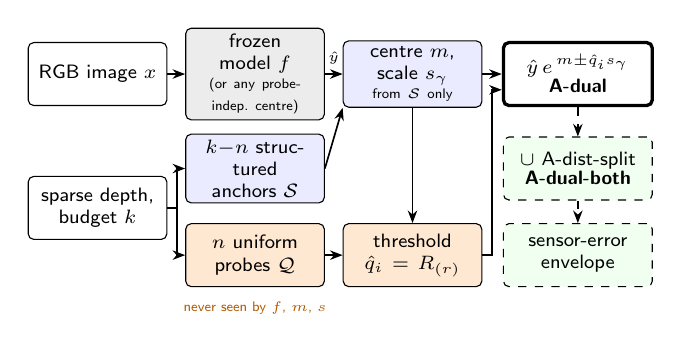
\begin{tikzpicture}[
  font=\sffamily\scriptsize,
  box/.style={draw, rounded corners=2pt, align=center, text width=1.62cm, minimum height=8mm, inner sep=2pt, fill=white},
  frozen/.style={box, fill=gray!15},
  anch/.style={box, fill=blue!8},
  prob/.style={box, fill=orange!18},
  outbox/.style={box, text width=1.75cm, fill=white, very thick},
  opt/.style={box, text width=1.75cm, dashed, fill=green!6},
  arr/.style={-{Stealth[length=1.6mm]}, semithick},
  darr/.style={-{Stealth[length=1.6mm]}, semithick, dashed}]
  % column 1: inputs
  \node[box]    (rgb)    at (0.85, 2.15) {RGB image $x$};
  \node[box]    (sensor) at (0.85, 0.45) {sparse depth,\\budget $k$};
  % column 2: model and split
  \node[frozen] (f)      at (2.85, 2.15) {frozen model $f$\\[-1pt]{\tiny(or any probe-indep.\ centre)}};
  \node[anch]   (S)      at (2.85, 0.95) {$k{-}n$ structured\\anchors $\cS$};
  \node[prob]   (Q)      at (2.85,-0.15) {$n$ uniform\\probes $\cQ$};
  % column 3: centre/scale and threshold
  \node[anch]   (ms)     at (4.85, 2.15) {centre $m$, scale $s_\gamma$\\[-1pt]{\tiny from $\cS$ only}};
  \node[prob]   (q)      at (4.85,-0.15) {threshold\\$\qhat_i=R_{(r)}$};
  % column 4: output and optional stages
  \node[outbox] (int)    at (6.95, 2.15) {$\yhat\,e^{\,m\pm\qhat_i s_\gamma}$\\[-1pt]\textbf{\mDual}};
  \node[opt]    (hull)   at (6.95, 0.95) {$\cup$ \mDistSplit\\[-1pt]\textbf{\mDualBoth}};
  \node[opt]    (env)    at (6.95,-0.15) {sensor-error\\envelope};
  % arrows
  \draw[arr] (rgb) -- (f);
  \draw[arr] (f) -- node[above, font=\tiny\sffamily]{$\yhat$} (ms);
  \draw[arr] (sensor.east) -- ++(0.12,0) |- (S.west);
  \draw[arr] (sensor.east) -- ++(0.12,0) |- (Q.west);
  \draw[arr] (S.east) -- (ms.south west);
  \draw[arr] (Q) -- (q);
  \draw[arr] (ms) -- (q);
  \draw[arr] (ms) -- (int);
  \draw[arr] (q.east) -- ++(0.12,0) |- ([yshift=-2mm]int.west);
  \draw[darr] (int) -- (hull);
  \draw[darr] (hull) -- (env);
  \node[font=\tiny\sffamily, text=orange!70!black, anchor=north] at (2.85,-0.62) {never seen by $f$, $m$, $s$};
\end{tikzpicture}
\caption{\textbf{Dual-role calibration.} Structured anchors $\cS$ build a centre $m$ and scale $s_\gamma$ around a frozen prediction $\yhat$ (or any probe-independent centre); the $n$ uniform probes $\cQ$ only score it and set one threshold per image (\cref{thm:dual}). Dashed: optional stages (\ifenvelopemain\cref{thm:both,prop:env}\else\cref{thm:both}; Supp.~D\fi).}
\label{fig:pipeline}
\end{figure}


\subsection{Architecture}
\label{sec:arch}
In the pipeline of \cref{fig:pipeline},
(1)~a frozen monocular model produces $\yhat$; nothing is retrained.
(2)~The sensor budget is split into $k-n$ anchors that follow the deployed layout and $n$ uniformly random probes.
(3)~The anchors alone build a local centre $m(p)$ and scale $s_\gamma(p)$ around $\yhat$ (\cref{sec:centre}).
(4)~The probes, unseen by stages 1--3, set one conformal threshold per image (\mDual, \cref{sec:dual}).
Optional stages add a per-distance-bin guarantee (\mDualBoth, \cref{sec:both}) and convert coverage of sensor readings into coverage of depth (\envref).
Stage~1 can be any predictor that does not see the probes, \eg a depth-completion network fed RGB and $\cS$; stage~3 is then refit around its output, so \mDual is a calibration layer, not a depth estimator.

\subsection{Centre and scale from structured anchors}
\label{sec:centre}
We use the distance-aware anchor model of the baseline \mDistSplit, fitted on the structured anchors only (details in Supp.~E).
For pixel $p$, the local shift $m(p)$ is one of four estimates from the anchor residuals $\dtil|_\cS$: the image median, the median of the 16 nearest anchors, or a Gaussian or bilateral (also weighting similarity in $\log\yhat$) kernel mean.
The local spread $\sigma(p)$ is the median absolute deviation of the 16 nearest anchor residuals, $\delta_\cS(p)$ is the distance to the nearest structured anchor as a fraction of the image diagonal, and
\begin{equation}
s(p)=\big(\sigma(p)+\tau\big)\,g\big(\delta_\cS(p)\big),
\label{eq:scale}
\end{equation}
with a floor $\tau$ and a non-decreasing $g$ fitted by isotonic regression of normalized error against distance.
The variant, bandwidths, $\tau$, $g$ and a cap on $s$ are chosen per layout on held-out \emph{head-train} images, never on calibration or test data.
The only property the guarantee below needs is that $m$ and $s$ are functions of $(x,\yhat,\cS,\dtil|_\cS)$, \ie that they do not depend on the probes.

\subsection{Per-image threshold from random probes (\mDual)}
\label{sec:dual}
When the anchors set the shift wrong everywhere, as a single cluster can, the residual is nearly flat, the threshold is set by the probes with the smallest $s$, and widths elsewhere grow by up to $\max s/\min s$.
We therefore shrink the scale toward its per-image median $M_i=\med_{p\in\cP_i}s(p)$:
\begin{equation}
s_\gamma(p)=M_i\,\big(s(p)/M_i\big)^{\gamma},\qquad \gamma=0.5 .
\label{eq:shrink}
\end{equation}
$s_\gamma$ depends on $s$ only, so it is as probe-independent as $s$.
For probes $\cQ=\{p_1,\dots,p_n\}$ with reported residuals $\dtil(p_j)$, define the scores and threshold
\begin{equation}
R_j=\frac{|\dtil(p_j)-m(p_j)|}{s_\gamma(p_j)},\quad
\qhat_i=R_{(r)},\quad r=\lceil(n+1)(1-\alpha)\rceil,
\label{eq:threshold}
\end{equation}
where $R_{(r)}$ is the $r$-th smallest score ($\qhat_i=\infty$ if $r>n$).
The interval at every evaluation pixel is
\begin{equation}
C(p)=\Big[\yhat(p)\,e^{\,m(p)-\qhat_i s_\gamma(p)},\;\yhat(p)\,e^{\,m(p)+\qhat_i s_\gamma(p)}\Big].
\label{eq:interval}
\end{equation}

\begin{theorem}[Dual-role validity]
\label{thm:dual}
Fix an image with valid pixels $\cP$ and a structured anchor set $\cS\subset\cP$ chosen by any rule, which may depend on $x$, $\yhat$ and the anchor values.
Let $m$, $s>0$ and $\gamma$ be determined by $(x,\yhat,\cS,\dtil|_\cS)$.
Let $v(p)$ be the log residual of the quantity the probes report ($v=d$ for exact depth, $v=\dtil$ for a sensor), defined on $\cU=\cP\setminus\cS$.
Draw $\cQ$ uniformly without replacement from $\cU$, compute $\qhat$ by \cref{eq:threshold} with $v$ in place of $\dtil$, and let $J$ be uniform on $\cU\setminus\cQ$.
Then
\begin{equation*}
\P\big(\yhat(J)e^{v(J)}\in C(J)\,\big|\,x,\cS,\dtil|_\cS\big)\;\ge\;\frac{r}{n+1}\;\ge\;1-\alpha,
\end{equation*}
with equality on the left when the scores have no ties and $r\le n$.
Equivalently, $\E[\Cov_i\mid x,\cS]\ge r/(n+1)$, the expectation taken over the probe draw.
\end{theorem}

\noindent\emph{Proof sketch.}
Given $(x,\cS,\dtil|_\cS)$, every $p\in\cU$ carries a fixed score $R(p)=|v(p)-m(p)|/s_\gamma(p)$, and the probes with $J$ form a uniformly random $(n+1)$-subset of $\cU$, so $R(J)$ is among the $r$ smallest of the $n+1$ scores, hence covered, with probability at least $r/(n+1)$. Supp.~A. \hfill$\square$

This is the split argument of~\cite{gui2023cmc,mao2024spatial} applied inside one image around a frozen prior; we claim no new theory.
It needs no calibration images and uses all $n$ probes for the threshold ($n\ge 9$ suffices at $\alpha=0.1$), whereas \mLocalSplit spends half on a shift.
\emph{Scope:} the guarantee holds in expectation over the probe draw, not per region; probes must be uniform over the pixels it concerns (\eg where the sensor returns); every choice, $\gamma$ included, is fixed without probe values; and it covers $v$, what the probes measure.

\subsection{Probe budget}
\label{sec:budget}
\Cref{thm:dual} fixes the mean of $\Cov_i$; $n$ fixes its spread.

\begin{proposition}[Per-image coverage law]
\label{prop:budget}
Under \cref{thm:dual} with no ties and $r\le n$, let $N=|\cU|$.
The number of covered evaluation pixels, $(N-n)\Cov_i$, follows exactly the beta-binomial law $\BetaBin(N-n,\,r,\,n+1-r)$.
As $N\to\infty$, $\Cov_i\to\BetaD(r,\,n+1-r)$ in distribution.
\end{proposition}

\noindent This is the finite-population form of the Beta law of split-conformal coverage conditional on the calibration set~\cite{vovk2012conditional}; with thousands of evaluation pixels per image the Beta approximation is excellent.
That measurements match this law (\cref{sec:res:budget}) is an implementation check implied by the randomization, not a finding.

\noindent\fbox{\parbox{\dimexpr\linewidth-2\fboxsep-2\fboxrule\relax}{\textbf{Design rule.}
The share of images below coverage $c$ in one draw is $\P(\BetaD(r,n{+}1{-}r)<c)=\P(\mathrm{Bin}(n,c)\ge r)$, known before any data are seen (\cref{tab:budget}).
At $\alpha=0.1$ it falls slowly with $n$ ($c=0.85$: \NumRuleShortHundred\% at $n=100$); the nominal level is the stronger lever: $n=r=20$ (nominal \NumRuleNomTwentyAll) leaves \NumRuleShortTwentyAll\% below 0.85 (measured on NYU and KITTI: \NumRmaxShort, coverage \NumRmaxCovLo--\NumRmaxCovHi), at \NumRmaxWidthCostLo--\NumRmaxWidthCostHi\% more width and \NumRmaxISCostLo--\NumRmaxISCostHi\% more interval score than $r=19$.}}

\begin{table}[t]
\centering\small
\setlength{\tabcolsep}{4pt}
\begin{tabular}{@{}rrccc@{}}
\toprule
$n$ & $r$ & $\frac{r}{n+1}$ & p10 of $\Cov_i$ & $\P(\Cov_i<0.85)$, \% \\
\midrule
10 & 10 & 0.909 & \NumBetaPTenTen   & \NumBetaShortOneTen \\
20 & 19 & 0.905 & \NumBetaPTenTwenty & \NumBetaShortOneTwenty \\
40 & 37 & 0.902 & \NumBetaPTenForty & \NumBetaShortOneForty \\
\bottomrule
\end{tabular}
\caption{\textbf{Probe budget at $\alpha=0.1$, one probe draw} (Beta approximation of \cref{prop:budget}; from the definition alone, no data).}
\label{tab:budget}
\end{table}

\subsection{Adding a per-distance-bin guarantee (\mDualBoth)}
\label{sec:both}
\mDual's coverage, in practice, decreases with distance to the nearest anchor.
The baseline \mDistSplit targets this: it fits the model of \cref{sec:centre} on all $k$ measurements and calibrates one threshold per bin of $\delta$ by conformal risk control~\cite{angelopoulos2024crc} over calibration \emph{scenes}, the loss being the miscovered fraction of bin pixels (a Mondrian construction~\cite{vovk2005alrw}; sparse bins are merged, Supp.~C).
For exchangeable scenes and the same anchor rule at calibration and test, the expected bin miscoverage of a new scene is at most $\alpha$ in every (merged) bin.
Unlike \mDual, this needs calibration scenes with dense depth from the same source as the measurements, and it certifies that source.
\mDualBoth is the pointwise hull
$C^{\text{both}}(p)=\big[\min(\ell^{\text{dual}},\ell^{\text{dist}}),\,\max(u^{\text{dual}},u^{\text{dist}})\big]$.

\begin{theorem}[Hull validity]
\label{thm:both}
\mDualBoth has the per-image guarantee of \cref{thm:dual} and the per-bin guarantee of \mDistSplit.
\end{theorem}

\noindent\emph{Proof sketch.} The hull contains each interval pointwise and both statements are monotone in the interval~\cite{gasparin2024merging}. Supp.~C. \hfill$\square$

\mDualBoth replaces \mDistBoth, the hull of \mDistSplit with \mLocalSplit. Any hull costs width, most when the two centres disagree, as under clustered anchors.

\ifenvelopemain
\subsection{Optional: sensor-error envelope}
\label{sec:env}
\TODO{gate: iPad-probe truth coverage $\ge0.9$ and IS $\ge$10\% below \mDistBoth, else \texttt{\textbackslash envelopemainfalse}.}
%% Sensor-error envelope: shared body of main Sec. 4.6 (\envelopemaintrue) and Supp. D (\envelopemainfalse).
%% Compiled in both documents, so it refers to Theorem 1 by its fixed main-paper number, not by \cref.
With sensor-valued probes, Theorem~1 certifies the reading $\ytil$, not the depth $y$.
Let $e(p)=\log\ytil(p)-\log y(p)$ and suppose a reference (here a laser scan) exists on calibration scenes.
We (a) subtract a global bias $\hat\beta$, the median of $e$ on head-train pixels, from the probe values, and (b) give each sensor-confidence class $c$ (ARKit: $0/1/2$) the band $[-a_c,b_c]=[Q_c(\lambda/2),Q_c(1-\lambda/2)]$ of the corrected head-train error, clipped to contain $0$.
One conformal risk control~\cite{angelopoulos2024crc} over the $U$ calibration scenes sets $\hat\lambda$: the largest grid value with $\frac{U}{U+1}\hat L(\lambda)+\frac{1}{U+1}\le\alpha_e$, $\hat L$ the mean fraction of a scene's pixels outside their band (none feasible: infinite bands).
With $[\ell,u]$ the \mDual interval for the corrected reading at level $1-\alpha_s$, the enveloped interval is
\begin{equation}
C^{\text{env}}(p)=\big[\ell(p)\,e^{-b_{c(p)}},\;u(p)\,e^{a_{c(p)}}\big].
\label{eq:envelope}
\end{equation}

\begin{proposition}[Envelope]
\label{prop:env}
If the sensor reading and its confidence are defined at every evaluation pixel, the miscoverage of $y$ by $C^{\text{env}}$, averaged over test scenes and probe draws, is at most $\alpha_s+\alpha_e$.
\end{proposition}

\ifenvelopemain
\noindent\emph{Proof sketch.} $y=\ytil e^{-\hat\beta}e^{-(e-\hat\beta)}$, so $y\notin C^{\text{env}}(p)$ requires either the corrected reading outside $[\ell,u]$ (probability at most $\alpha_s$ per image, Theorem~1) or the corrected error outside its band (at most $\alpha_e$ in expectation, by risk control); a union bound concludes. Supp.~D. \hfill$\square$

\fi
The per-image guarantee on $y$ is not retained: the envelope's part holds on average over scenes.
We fix $\alpha_s=\alpha_e=0.05$ before the run, so that $\alpha_s+\alpha_e=\alpha$.

\else
\paragraph{Sensor-valued probes.} With sensor-valued probes, \cref{thm:dual} certifies the reading; an optional sensor-error envelope that converts this into an average-over-scenes guarantee on depth is given in Supp.~D; it restored truth coverage here (\NumEnvTruthCov{} with iPad probes) but at a higher interval score than \mDistBoth.
\fi

\section{Experimental setup}
\label{sec:experiments}

\paragraph{Datasets.}
\emph{NYU Depth v2}~\cite{silberman2012nyu}: 1{,}449 images from 464 rooms (Kinect, $<$10\,m).
\emph{KITTI}~\cite{geiger2012kitti}: 652 Eigen test plus 800 Eigen-train frames from 61 drives (Garg crop, $<$80\,m); its ground truth comes from the LiDAR that would provide the anchors, so it cannot test an independent sensor.
\emph{ARKitScenes}~\cite{baruch2021arkitscenes}, depth-upsampling validation split: \NumArkFrames{} frames from \NumArkVisits{} visits, ground truth from a Faro laser scan, deployed sensor the iPad Pro LiDAR depth from ARKit (fused, with confidence $\{0,1,2\}$), which reads about \NumArkIpadOffset\% nearer than the laser (preprocessing in Supp.~G).
Valid pixels are kept on a lattice (stride 4 on NYU, 2 on KITTI, 8 on ARKitScenes) and stored per image, so per-image statistics are exact.
Every split is by scene (room, drive, visit): 30\% head-train (fits $m$, $s$ and hyper-parameters), 35\% calibration (cross-scene thresholds; unused by \mDual), 35\% test.

\paragraph{Frozen models.}
UniDepthV2-Large~\cite{piccinelli2025unidepthv2}, Depth Anything V2 Large metric~\cite{yang2024dav2} (indoor checkpoint, fine-tuned on Hypersim, on NYU and ARKitScenes; outdoor checkpoint, fine-tuned on Virtual KITTI~2, on KITTI) and, on NYU and KITTI, Depth Pro~\cite{bochkovskii2025depthpro}; Metric3D v2~\cite{hu2024metric3dv2} is in the supplement.
NYU and KITTI are not in the training mixtures of these models (Supp.~G).
UniDepthV2's training mixture includes ARKitScenes (split not reported)~\cite{piccinelli2025unidepthv2}; our validation-split frames are likely unseen, the domain is not, which affects width, not any guarantee.
Depth Pro, trained on ARKitScenes, is not used there.

\paragraph{Measurements.}
$k\in\{50,200\}$ measurements per image, of which $n=20$ are probes (ablation $n\in\{10,40\}$), under the five layouts of \cref{sec:setup}.
On NYU and KITTI they report the ground truth.
On ARKitScenes, anchors and probes each report the laser or the iPad value, a $2\times2$ factorial (laser/laser, iPad/laser, laser/iPad, iPad/iPad); coverage is always measured against the laser.
For UniDepthV2 and DA-V2 (E18): $k=200$ (180 anchors, 20 probes), uniform and cluster layouts, \NumReplSplits{} visit splits $\times$ \NumProbeDraws{} probe draws.

\paragraph{Methods.}
All methods share positions and the log-residual score.
\emph{Baselines:} \mLocal~\cite{mao2024spatial} calibrates within the image on the structured anchors themselves (half fix a shift, half set the width; valid only for uniform anchors); \mLocalSplit does the same on the $n$ probes; \mDistSplit (\cref{sec:both}); \mDistBoth $=$ hull(\mDistSplit, \mLocalSplit).
\emph{Ours:} \mDual\ifenvelopemain, \mDualBoth and \mDualEnv\else{} and \mDualBoth\fi.
\emph{Completion centre (E19):} \omnidc~\cite{zuo2025omnidc} (v1.1, Depth Anything V2 prior; trained only on five synthetic datasets, Hypersim, IRS, TartanAir, BlendedMVS and Virtual KITTI, so zero-shot on ARKitScenes) on ARKitScenes, $k=200$ (180 anchors, 20 probes), uniform and cluster layouts, laser anchors with laser or iPad probes (iPad-anchor cells: exploratory, three splits), UniDepthV2 as the frozen alternative, \NumOmniSeeds{} visit splits $\times$ 1 probe draw.
\omnidc sees RGB and the structured anchors only, never the probes.
Both centres are calibrated four ways: \mSplitCP (one quantile of $|\log y-\log\yhat|$ over calibration-scene pixels; marginal; needs dense laser depth), \mDistSplit, \mDual and \mDualBoth, with $m$, $s$ refit per centre.

\paragraph{Metrics.}
Coverage is image-averaged \cref{eq:cov}; per-image spread is the 10th percentile (p10) of $\Cov_i$ and the share of \emph{short} images, whose coverage on one probe draw is below $1-\alpha-0.05=0.85$ (law: \NumBetaShortOneTwenty\% at $n=20$).
Width is the median of $(u-\ell)/\yhat$, or of $(u-\ell)/y$ when centres differ.
The pixel interval score $(u-\ell)+\tfrac{2}{\alpha}\big[(\ell-y)_+ + (y-u)_+\big]$ penalizes misses by their size; the relative interval score is the median over images of its per-image mean over $y$, robust to a few extreme images while keeping the miss penalty (exploratory: mean over images); the share of pixels with intervals wider than $10y$ (infinite included) exposes failures a robust score hides.

\paragraph{Protocol.}
$\alpha=0.1$ throughout.
Exploratory runs (3 scene splits $\times$ 2 probe draws; E18: \NumReplSplits{} splits; E19: 3 splits $\times$ 1 draw) chose the shrinkage $\gamma=0.5$ (\cref{eq:shrink}), after $\gamma=1$ showed a heavy width tail, and the design; validity holds for any fixed $\gamma$.
All reported comparisons come from a confirmatory replication whose analysis plan was fixed before the runs: \NumReplSplits{} splits $\times$ \NumProbeDraws{} draws on NYU and KITTI (plus an $r=n=20$ arm) and in E18; in E19, 10 splits with their own anchor masks and \omnidc from laser anchors (Supp.~G).
A method is valid if its mean coverage is $\ge1-\alpha-2\,$SE (\mDual: also within 2\,SE of $r/(n+1)$), and better only if the 95\% paired bootstrap interval over splits ($10^4$ resamples) of the IS difference excludes zero.

\section{Results}
\label{sec:results}

\placeholder{remaining exploratory numbers}{E17, E18, E19 (laser anchors) and E20 are confirmatory. Orange numbers are exploratory (\cref{sec:experiments}): the motivation numbers of \cref{sec:res:failure} beyond \cref{tab:main}, the probe-count ablation, and E19 with iPad anchors; E19 table cells are still rendered orange.}

%% ---------------------------------------------------------------- Table 2 (NYU/KITTI)
\begin{table}[t]
\centering\footnotesize
\setlength{\tabcolsep}{3pt}
\newcommand{\rowE}[3]{#1 & #3 & \ESeventeen{#2}{#3}{local} & \ESeventeen{#2}{#3}{dual} & \ESeventeen{#2}{#3}{short} & \ESeventeen{#2}{#3}{dW} & \ESeventeen{#2}{#3}{bW} & \ESeventeen{#2}{#3}{dIS} & \ESeventeen{#2}{#3}{bIS} \\}
\begin{tabular}{@{}llccccccc@{}}
\toprule
 & & \multicolumn{2}{c}{Coverage} & Short (\%) & \multicolumn{2}{c}{$\Delta$ width (\%)} & \multicolumn{2}{c}{$\Delta$ IS (\%)} \\
\cmidrule(lr){3-4}\cmidrule(lr){5-5}\cmidrule(lr){6-7}\cmidrule(l){8-9}
Layout & $k$ & \textsf{local} & \textsf{dual} & \textsf{dual} & \textsf{dual} & \textsf{both} & \textsf{dual} & \textsf{both} \\
\midrule
\rowE{uniform}{uniform}{50}\rowE{}{uniform}{200}
\midrule
\rowE{rows}{rows}{50}\rowE{}{rows}{200}
\midrule
\rowE{cluster}{cluster}{50}\rowE{}{cluster}{200}
\midrule
\rowE{edges}{edges}{50}\rowE{}{edges}{200}
\midrule
\rowE{near}{near}{50}\rowE{}{near}{200}
\midrule
\multicolumn{2}{@{}l}{theory} & $\ge$0.9$^\dagger$ & \NumDualCovTheory & \NumBetaShortOneTwenty$^\ddagger$ & & & & \\
\bottomrule
\end{tabular}
\caption{\textbf{NYU and KITTI, three frozen models, $n=20$ probes, $\alpha=0.1$}; confirmatory, \NumReplSplits{} scene splits $\times$ \NumProbeDraws{} probe draws; median over the six model--dataset pairs (ranges in the supplement). \textsf{local}: \mLocal calibrated on the $k$ structured anchors themselves; \textsf{dual}: \mDual; \textsf{both}: \mDualBoth. Short: \% of images whose coverage on one probe draw is below 0.85. $\Delta$: change in median relative width and relative interval score (IS, primary) against \mDistBoth. $^\dagger$Uniform anchors only. $^\ddagger$\Cref{tab:budget}.}
\label{tab:main}
\end{table}

%% ---------------------------------------------------------------- Figure 3
\begin{figure}[t]
\centering
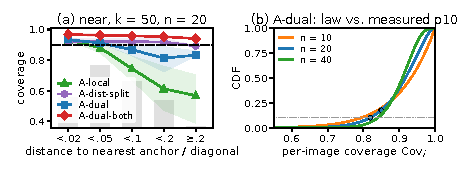
\includegraphics[width=\linewidth]{figures/e17_results.pdf}
\caption{\textbf{What each guarantee protects.} (a)~Near layout, $k=50$, $n=20$: \mDual's coverage decreases with distance, as \cref{thm:dual} allows; \mDualBoth is flat. Lines/bands: median/range over the six NYU/KITTI pairs; bars: pixel share; dashed: 0.9. (b)~CDF of the per-image coverage law (\cref{prop:budget}), $n=10,20,40$; dots at 0.1: measured p10 of $\Cov_i$ (median over pairs, layouts, $k$); dot at 0.85: measured share of short images, $n=20$. Confirmatory for $n=20$ (\NumReplSplits{} splits $\times$ \NumProbeDraws{} draws); $n=10,40$ exploratory.}
\label{fig:results}
\end{figure}

\subsection{Structured anchors break reused calibration}
\label{sec:res:failure}
Calibrating within the image on the structured anchors themselves (\cref{tab:main}, \textsf{local}) keeps nominal coverage only for uniform anchors.
Under clustered anchors it covers \ESeventeen{cluster}{50}{local} and \ESeventeen{cluster}{200}{local} at $k=50$ and $200$, under near-only anchors \ESeventeen{near}{50}{local} and \ESeventeen{near}{200}{local}, and under scan lines \ESeventeen{rows}{200}{local} at $k=200$; edge anchors over-cover, since edges are where errors are largest.
The failing intervals are narrower, not wider: with 20 clustered anchors their median relative width was \NumLocalClusterWidthLo--\NumLocalClusterWidthHi{} against \NumLocalUnifWidthLo--\NumLocalUnifWidthHi{} for uniform ones.
Even uniform anchors hide a spatial gap: coverage fell from \NumLocalNearBinCovLo--\NumLocalNearBinCovHi{} next to an anchor to \NumLocalFarBinCovLo--\NumLocalFarBinCovHi{} beyond 0.2 of the diagonal.

\subsection{Separating the roles restores per-image validity}
\label{sec:res:dual}
\mDual covers \NumDualCovLo--\NumDualCovHi{} in every layout, $k$ and pair, at its theoretical rate $r/(n+1)=\NumDualCovTheory$ (within two standard errors in \NumDualExactCells{} of the \NumAllCells{} pair--layout--$k$ cells), and is at least 10\% narrower than \mDistBoth on \NumDualGatePairs{} of \NumPairs{} pairs in each of the \NumCells{} layout--$k$ cells (\cref{tab:main}; paired bootstrap intervals exclude 0).
Part of that width is \mDistBoth's over-coverage (\NumDistBothCovLo--\NumDistBothCovHi), so the interval score, which charges misses, is the fairer comparison.
On it \mDual is better in \NumDualISWins{} of the \NumAllCells{} cells, including every cell with uniform or scan-line anchors (by \NumDualISGainURLo--\NumDualISGainURHi\%); \mDistBoth is better in \NumDualISLosses, nine of them clustered, by at most \NumDualISLoseMax\%.
\mDualBoth is better than \mDistBoth in \NumDualBothISWins{} cells and worse in \NumDualBothISLosses, all clustered and by at most \NumDualBothISLoseMax\%; under clustered anchors its halves are centred differently and it gains only \NumDualBothClusterWidthLo--\NumDualBothClusterWidthHi\% in width.
\mDual's coverage varies across distance bins by \NumSpreadDualLo--\NumSpreadDualHi{} points; \mDualBoth reduces this to \NumSpreadDualBothLo--\NumSpreadDualBothHi{} (\cref{fig:results}a).

\subsection{The probe budget}
\label{sec:res:budget}
With 20 probes the 10th percentile of $\Cov_i$ was \NumMeasPTenTwenty{} (law: \NumBetaPTenTwenty) and \NumESeventeenShort{} of images were short in one draw (law: \NumBetaShortOneTwenty\%), an implementation check (\cref{fig:results}b).
With 10 probes \mLocalSplit, hence \mDistBoth, is infinite on every image (5 calibration probes, fewer than the 9 needed), while \mDual stays finite at median width \NumWDualTenFifty/\NumWDualTenTwoHundred{} ($k=50/200$).
In exploratory runs with 40 probes, the share of images short on average over two draws fell to \NumShortFortyLo--\NumShortFortyHi\% (law: \NumBetaShortTwoForty\%) at similar width (\NumWDualFortyFifty/\NumWDualFortyTwoHundred), but under clustered anchors \mDual misses the 10\% margin over \mDistBoth. We keep $n=20$.

%% ---------------------------------------------------------------- Table 3 (ARKitScenes, E19)
\begin{table*}[t]
\centering\footnotesize
\setlength{\tabcolsep}{2.5pt}
\newcommand{\eA}[3]{\ENineteen{#1}{#2}{clean}{clean}{#3}{cov} & \ENineteen{#1}{#2}{clean}{clean}{#3}{ptten} & \ENineteen{#1}{#2}{clean}{clean}{#3}{short} & \ENineteen{#1}{#2}{clean}{clean}{#3}{wgt} & \ENineteen{#1}{#2}{clean}{clean}{#3}{is}}
\newcommand{\rowA}[3]{#1 & #3 & \eA{uniform}{#2}{#3} & \eA{cluster}{#2}{#3} \\}
\newcommand{\eB}[3]{\ENineteen{#1}{#2}{clean}{clean}{#3}{cov} & \ENineteen{#1}{#2}{lidar}{clean}{#3}{cov} & \ENineteen{#1}{#2}{clean}{lidar}{#3}{cov} & \ENineteen{#1}{#2}{lidar}{lidar}{#3}{cov}}
\newcommand{\rowB}[3]{#1 & #3 & \eB{uniform}{#2}{#3} & \eB{cluster}{#2}{#3} \\}
\newcommand{\eC}[3]{\EEighteen{#1}{#2}{clean}{clean}{#3}{cov} & \EEighteen{#1}{#2}{lidar}{clean}{#3}{cov} & \EEighteen{#1}{#2}{clean}{lidar}{#3}{cov} & \EEighteen{#1}{#2}{lidar}{lidar}{#3}{cov}}
\newcommand{\rowC}[3]{#1 & #3 & \eC{uniform}{#2}{#3} & \eC{cluster}{#2}{#3} \\}
\ifenvelopemain
\newcommand{\envrow}{ & \mDualEnv & -- & -- & \pending{env} & \pending{env} & -- & -- & \pending{env} & \pending{env} \\}
\else
\newcommand{\envrow}{}
\fi
\textbf{(a) Laser-valued anchors and probes: which centre to calibrate}\\[2pt]
\begin{tabular}{@{}llccccc@{\hspace{5pt}}ccccc@{}}
\toprule
 & & \multicolumn{5}{c}{Uniform layout} & \multicolumn{5}{c}{Cluster layout} \\
\cmidrule(lr){3-7}\cmidrule(l){8-12}
Centre & Calib. & Cov. & p10 & Short\,\% & W$/y$ & IS & Cov. & p10 & Short\,\% & W$/y$ & IS \\
\midrule
UniDepthV2 & \mSplitCP & \eA{uniform}{unidepth}{split-CP} & \eA{cluster}{unidepth}{split-CP} \\
\midrule
\rowA{UniDepthV2 + $\cS$}{unidepth}{A-dist-split}
\rowA{}{unidepth}{A-dual}
\rowA{}{unidepth}{A-dual-both}
\midrule
\rowA{\omnidc + $\cS$}{omnidc}{split-CP}
\rowA{}{omnidc}{A-dist-split}
\rowA{}{omnidc}{A-dual}
\rowA{}{omnidc}{A-dual-both}
\midrule
\multicolumn{2}{@{}l}{theory, one draw} & \NumDualCovTheory & \NumBetaPTenTwenty & \NumBetaShortOneTwenty & & & \NumDualCovTheory & \NumBetaPTenTwenty & \NumBetaShortOneTwenty & & \\
\bottomrule
\end{tabular}\\[6pt]
\textbf{(b) Laser-truth coverage by value source of anchors / probes (L = laser, I = iPad LiDAR)}\\[2pt]
\begin{tabular}{@{}llcccc@{\hspace{14pt}}cccc@{}}
\toprule
 & & \multicolumn{4}{c}{Uniform layout} & \multicolumn{4}{c}{Cluster layout} \\
\cmidrule(lr){3-6}\cmidrule(l){7-10}
Centre & Calib. & L/L & I/L & L/I & I/I & L/L & I/L & L/I & I/I \\
\midrule
\rowC{UniDepthV2 + $\cS$}{unidepth}{A-dist-split}
\rowC{}{unidepth}{A-dual}
\rowC{}{unidepth}{A-dist-both}
\envrow
\midrule
\rowC{DA-V2 + $\cS$}{dav2}{A-dual}
\midrule
\rowB{\omnidc + $\cS$}{omnidc}{split-CP}
\rowB{}{omnidc}{A-dist-split}
\rowB{}{omnidc}{A-dual}
\bottomrule
\end{tabular}
\caption{\textbf{ARKitScenes, $k=200$ ($180$ structured anchors $+$ $20$ probes), $\alpha=0.1$.} (a) and the \omnidc rows of (b): E19, UniDepthV2 frozen, mean over \NumOmniSeeds{} visit splits, one probe draw (confirmatory; \omnidc with iPad anchors, I/L and I/I: exploratory, three splits). Frozen-model rows of (b): E18, mean over \NumReplSplits{} visit splits and \NumProbeDraws{} probe draws (confirmatory). Coverage is always of the laser ground truth. p10 and short: 10th percentile of per-image coverage and \% of images below 0.85, for a single probe draw. W$/y$: median width over laser depth; IS: relative interval score (\cref{sec:experiments}). \omnidc sees RGB and the structured anchors only, never the probes. \mSplitCP calibrates on dense laser depth of calibration scenes; \mDistSplit on the values the measurements report. Under clustered anchors, 0.1--0.4\% of \omnidc pixels with extreme upper bounds dominate a mean over images, not the IS shown (Supp.~G). Full grid in the supplement.}
\label{tab:arkit}
\end{table*}

\subsection{Which centre to calibrate}
\label{sec:res:omni}
\emph{Uniform anchors.} \omnidc is the better centre: \mSplitCP, \mDual and \mDistSplit on its output have a \NumOmniGainLo--\NumOmniGainHi\% lower interval score than \mDual on UniDepthV2 (paired intervals exclude zero), which fires the criterion we fixed before the run ($\ge$15\%), so the layer belongs on top of the completion network.
\mDual with \omnidc as centre costs \NumOmniDualCost\% in interval score over \mSplitCP on the same output and adds the per-image law: p10 \ENineteen{uniform}{omnidc}{clean}{clean}{A-dual}{ptten} and \ENineteen{uniform}{omnidc}{clean}{clean}{A-dual}{short}\% short images in one draw, as \cref{tab:budget} predicts.
\mSplitCP's spread is similar here (\ENineteen{uniform}{omnidc}{clean}{clean}{split-CP}{short}\% short) but carries no per-image guarantee, and it needs dense reference depth on calibration scenes.
\mDistSplit on \omnidc is the most efficient (\ENineteen{uniform}{omnidc}{clean}{clean}{A-dist-split}{is}) but has no per-image guarantee and, under uniform anchors, fails with sensor-valued anchors (\cref{sec:res:sensor}).
Without anchors, \mSplitCP on the frozen model has \NumRawRatioLo--\NumRawRatioHi$\times$ the interval score of any anchored method.

\emph{Clustered anchors.} The ranking reverses.
Away from one observed patch the completion network extrapolates poorly (AbsRel 0.074, vs.\ 0.039 for UniDepthV2 rescaled by the same anchors; Supp.~G): \mSplitCP on its output falls short of validity (coverage \ENineteen{cluster}{omnidc}{clean}{clean}{split-CP}{cov}, more than 2\,SE below 0.9) with p10 \ENineteen{cluster}{omnidc}{clean}{clean}{split-CP}{ptten} and \ENineteen{cluster}{omnidc}{clean}{clean}{split-CP}{short}\% short images, and \mDual on UniDepthV2 has a \NumClusterGainDual\% lower interval score than \mDual on \omnidc (\NumClusterGainCP\% lower than \mSplitCP on \omnidc, where \mDual beats \mSplitCP by 17\%).
The monocular prior carries the far field and the anchors fix its scale; this holds over \NumOmniSeeds{} splits, for one network and one dataset.
On this centre \mDistSplit is more efficient still (\ENineteen{cluster}{unidepth}{clean}{clean}{A-dist-split}{is}), without a per-image guarantee; \mDualBoth keeps both guarantees at \ENineteen{cluster}{unidepth}{clean}{clean}{A-dual-both}{is}.
Across both centres and layouts, \mDual's per-image spread is the same (p10 \NumENineteenPTenLo--\NumENineteenPTenHi, \NumENineteenShortLo--\NumENineteenShortHi\% short), as \cref{thm:dual} requires of any probe-independent centre.
\subsection{What the probes certify: an independent sensor}
\label{sec:res:sensor}
\Cref{tab:arkit}b (E18, confirmatory) varies what the measurements report, for UniDepthV2 and DA-V2 (AbsRel \NumArkUniAbsRel{} and \NumArkDavAbsRel) over \NumReplSplits{} visit splits $\times$ \NumProbeDraws{} draws, on data not used to choose $\gamma$.
With laser values for both, \mDual covers \NumEEighteenCovLL{} with the predicted spread.
With iPad anchors and laser probes, it covers the laser truth at \NumEEighteenCovIL{} in both layouts with the same spread (p10 \NumEEighteenPTen, short \NumEEighteenShort{} over both cells), because the probes measure the truth and absorb the anchors' bias into the threshold.
\mDistSplit, calibrated on the values the measurements report, covers it at only \NumEEighteenDistIpad{} under uniform anchors; its wider cluster bins absorb the bias (\NumEEighteenDistIpadCluster).
With laser anchors and iPad probes, \mDual over-covers (\NumEEighteenCovLI{} uniform, \NumEEighteenCovLICluster{} cluster), with \NumEEighteenWiden$\times$ wider intervals under uniform anchors, as the iPad's own errors enter the threshold.
With iPad values for both, the deployed configuration without a reference, \mDual certifies the iPad reading.
Under uniform anchors its intervals are about as narrow as the \NumArkIpadOffset\% sensor bias, and it covers the laser truth at only \NumEEighteenCovII{} (p10 \NumEEighteenPTenII, short \NumEEighteenShortII; \omnidc: \ENineteen{uniform}{omnidc}{lidar}{lidar}{A-dual}{cov}); the wider cluster intervals absorb more (\NumEEighteenCovIICluster), and the hull \mDualBoth recovers the truth there (\NumEEighteenHullIICluster) but not under uniform anchors (\NumEEighteenHullII).
Earlier within-image methods do the same (iPad anchors: \mLocal{} \NumArkLocalIpadCovUni, LSCP~\cite{jiang2024lscp} \NumArkLscpIpadCovUni).
Two methods cover the truth in every cell: \mSplitCP, because it calibrates on laser depth of other scenes, which a deployed system lacks, and \mDistBoth (at least \NumEEighteenDistBothMin) through width, at \NumEEighteenDistBothRatio$\times$ \mDual's interval score under uniform anchors with laser values.
Probes certify what they measure\ifenvelopemain; sensor-grade probes need \cref{sec:env}.

\placeholder{envelope, not yet run}{fills the \mDualEnv row; if the gate fails, set \texttt{\textbackslash envelopemainfalse}.}
\else.
The envelope of Supp.~D restores truth coverage with iPad probes (\NumEnvTruthCov) but over-covers, at an interval score \NumEnvISWorse{} above \mDistBoth's.
\fi

\section{Limitations}
\label{sec:limitations}

\emph{Expectation, not every draw:} with 20 probes about \NumBetaShortOneTwenty\% of images fall below 0.85 coverage in a single draw (\cref{tab:budget}).
\emph{No spatial guarantee from probes alone:} the per-distance guarantee of \mDualBoth needs calibration scenes and the same anchor rule at deployment.
\emph{What is certified:} the probes' quantity (\cref{sec:res:sensor}); \ifenvelopemain the envelope that would fix this holds only on average over scenes.\else with sensor-grade probes our truth guarantee comes only through width: the envelope of Supp.~D holds on average over scenes, not per image, and costs more than \mDistBoth.\fi{} ARKit depth is fused and dense; raw sparse returns and dropouts on glass or sky are untested.
\emph{The centre:} under uniform anchors a completion network is better; our centre's advantage under clusters rests on one network, one dataset and \NumOmniSeeds{} splits.
\emph{Selection of $\gamma$} used NYU and KITTI, so only ARKitScenes checks efficiency on held-out data; UniDepthV2 saw ARKitScenes in training.
\emph{Scope:} one $\alpha$, two budgets, one independent sensor, uniform probes by design (with a fixed-pattern scanner the guarantee covers only pixels with a return), and no downstream use: we do not show that the intervals improve an AR or planning task; active placement is not studied.

\section{Conclusion}
\label{sec:conclusion}

Structured sparse measurements make monocular foundation models far more accurate per image, but reused as calibration data they silently void the per-image guarantee.
Giving the sensor budget two roles fixes this: structured anchors build the prediction, and a few uniformly random probes, hidden from the predictor, calibrate it within each image.
The resulting layer needs no calibration images, makes the probe count a design parameter, and runs on any probe-independent centre.
It certifies what the probes measure: laser probes certified the depth even with iPad anchors, iPad probes only the iPad reading.

{
    \small
    \bibliographystyle{ieeenat_fullname}
    \bibliography{refs}
}

\end{document}
